\input{HeaderPRX.tex}

\begin{document}

% The following information is for internal review, please remove them for submission
\widetext
\leftline{Version xx as of \today}
\leftline{Primary authors: Joe E. Physics}
\leftline{To be submitted to PRX}
\leftline{Comment to {\tt d0-run2eb-nnn@fnal.gov} by xxx, yyy}
\centerline{\em D\O\ INTERNAL DOCUMENT -- NOT FOR PUBLIC DISTRIBUTION}

% the following line is for submission, including submission to the arXiv!!
%\hspace{5.2in} \mbox{Fermilab-Pub-04/xxx-E}

\title{Gauging defects in quantum spin systems}
\input author_list.tex       % D0 authors (remove the first 3 lines
                             % of this file prior to submission, they
                             % contain a time stamp for the authorlist)
                             % (includes institutions and visitors)
\date{\today}


\begin{abstract}
% !TEX root = Notes_Gauging_Defects.tex
The goal of this work is to build a dynamical theory of defects for quantum spin systems. A kinematic theory for an indefinite number of defects is first introduced exploiting \emph{distinguishable Fock space}. Dynamics are then incorporated by allowing the defects to become mobile via a microscopic Hamiltonian. This construction is extended to topologically ordered systems by restricting to the ground state eigenspace of Hamiltonians generalizing the \emph{golden chain}. We illustrate the construction with the example of a spin chain with $\Vec(\Z/2\Z)$ fusion rules, employing generalized tube algebra techniques to model the defects in the chain. The resulting dynamical defect model is equivalent to the critical transverse Ising model.
\end{abstract}

\pacs{}
\maketitle

\section{Introduction}
% This line sets the project root file.
% !TEX root = Notes_Gauging_Defects.tex
% !TEX spellcheck = en_US

Many important discoveries in condensed matter physics during the past decades have arisen from the study of \emph{topological states of matter} (see, for example, \cite{Wen07,NSSFD08,HK10,QZ11}). For a long time it was thought that all continuous phase transitions could be described by the Ginzburg-Landau theory of symmetry breaking. In the late 1980s, however, physicists discovered that some systems can exhibit a new kind of order going beyond the usual symmetry breaking paradigm. This new kind of order -- \emph{topological order} \cite{Wen90} -- soon became an interesting topic in its own right, useful for the description of different quantum Hall states \cite{WN90}. More recently, topologically ordered systems gave rise to \emph{topological quantum computation}, because of their remarkable properties: these locally interacting systems exhibit emergent global properties protected against environmental noise. This makes them a promising platform for the robust encoding, storage, and manipulation of quantum systems \cite{DKLP2002,Kit03,NSSFD08,Ter15,PY15,BLPSW16}.

However, in many phases, which includes those most suitable for experimental realization, the quantum computational power of a topologically ordered system is severely limited. To ameliorate this, defects in topologically ordered systems were considered \cite{RH07,Bombin2010,KK12,FSV13,BJQ13b,BASP14,JPSV15,DIP16,CCW16,BBD17,CCW17b,CCW17,BLKW17,KPEB18,ET19}, since a theory which includes defects can describe topological phases with enhanced computational power \cite{Freedman1998,FLW02b,FLW02,FKLW02}. For example, it is possible to use topologically ordered systems which are not universal for quantum computation to realize a computationally universal braiding gate set by adding defects \cite{BJQ13}.

In condensed matter physics, there is another approach to adding defects, which even in the case of simple and well-understood quantum systems substantially enriches their physics. Consider a simple example of fermions moving freely in one spatial dimension: the addition of a single defect -- an \emph{impurity} -- leads to a substantially richer and more complex system exhibiting Kondo-type effects \cite{andersonLocalizedMagneticStates1961,hewsonKondoProblemHeavy1997}. The study of such impurity models by Wilson \cite{wilsonRenormalizationGroupCritical1975} directly led to the revolutionary development of the density matrix renormalization group (DMRG) \cite{whiteDensityMatrixFormulation1992}, and the subsequent tensor network revolution \cite{bridgemanHandwavingInterpretiveDance2017}.

In the presence of additional symmetries, the phases of quantum systems have an even finer classification \cite{Wen2002,SRFL08,Kitaev2009,FK10,CGW11,FK11,TPB11,LS12,LV12,FM13,EH13,NCMT14,WPS14,K14,F14,EN14,MFCV15,BRSX15,LV16}. More precisely, it is possible for two quantum states that are equivalent when there is no additional symmetry present to be distinct in the presence of additional symmetries. This phenomenon is referred to as \emph{symmetry-protected topological} order (SPT) \cite{CGLW13,Yoshida2015,Yoshida2017} if the gapped phase is trivial in the absence of any symmetry, or as \emph{symmetry-enriched topological} (SET) order \cite{ENO10,MR13,WBV17} if the phase is topologically nontrivial. As far as defects are concerned, not only the distinct phases of matter acquire a finer classification in the presence of additional symmetries, but also the class of possible defects becomes larger. 

It is possible to to transform a topologically ordered system in the presence of a global symmetry to a system with a local gauge invariance. This is referred to as ``gauging the symmetry''. This is convenient for several reasons. For example, many properties of the ungauged system can be understood by looking at the properties of the gauged theory \cite{LG12,HW12,Swingle2014,CG14}. Furthermore, it may give insights into the quantum phase transitions between two different topological phases of matter \cite{BS09,BW10,BW11,BSS12}. 
The study of the fusion properties of defects in general quantum phases -- particularly when they are allowed to be mobile -- is deeply connected with global and local symmetries and the formalism of \emph{G-crossed braided tensor categories} \cite{BBCW14}. This connection has been studied from a mathematical point of view in various works \cite{T00,ENO10,Turaev2010,CGPW16,EMJP18,CSZW18,D19,BJ19}. The study of models involving mobile defects -- analogues of impurity models for anyons -- with nontrivial dynamics lies at the very cutting edge of current research. Such models promise to provide new phases of matter even in $(1+1)$ dimensions, going beyond the SPT classification.

In our work, the goal is to make physical and microscopic sense of a dynamical theory of defects for a one-dimensional quantum spin chain with $\Vec(\Z/2\Z)$ fusion rules. While we are focusing on this particular case study, the framework we establish can easily be extended to arbitrary quantum spin chains. Define the kinematical data for the system with an indefinite number of defects is straightforward via the well-known Fock space construction, whereas imposing dynamics is more complicated. In the context of topologically ordered systems, such as the considered $\Vec(\Z/2\Z)$ spin chain, dynamical information is typically introduced via the ground eigenspace of a specific Hamiltonian that represents the topological properties of the system. A common example is Kitaev's toric code for $N\times N$ quantum spins arranged on the torus, which exhibits a four-dimensional ground eigenspace. Defects in this system could be modeled by absent quantum spins, resulting in ground eigenspaces of differing dimensions. When considering more than one defect (i.e., missing spins) one also has to distinguish between cases where the defects are next to each other and those where they are spatially separated. This can result in a complicated combinatorial problem as shown in Subsec.~\ref{Kin_Dyn}. Therefore, we use tools from category theory to simplify explicit computations.

In our particular example of the one-dimensional example of a $\Vec(\Z/2\Z)$ spin chain defects are modeled by an invertible bimodule of the underlying category, see Subsec.~\ref{subsec:VecZ2}.
Using generalized tube algebra techniques \cite{ocneanu}, we construct explicit trivalent vertices for the gauged theory. Consistent with the literature \cite{TY,ENO10,Bombin2010,BBCW14,WBV17}, we find that the $F$-symbols of the gauged theory (computed using these explicit vertices) coincide exactly with those of the Ising category. To the best of our knowledge, this is the first time such a result has been computed directly using the tube algebra. Furthermore, defining a golden-chain-like Hamiltonian \cite{Feiguin2007} for this spin chain results in the transverse Ising model.

This paper is structured as follows: In Sec.~\ref{S:defs}, we provide definitions and background required for the remainder of the paper. We start by showing how to construct the Hilbert space for a quantum spin system in the presence of defects. This is followed by a recap on how to incorporate dynamics to these systems in the presence of topological order. By briefly studying the simple example of Kitaev's toric code it becomes clear that this task ends up in an extremely cumbersome combinatorial exercise. That is why we will need to introduce the language of category theory to continue our studies. In particular, we need the concepts from generalized tube algebras provided here to be able to study explicit examples of models with dynamical defects. In Sec.~\ref{Ising}, we transfer the previously introduced concepts to a spin chain with $\Vec(\Z/2\Z)$ fusion rules, which enables us to compute its dynamical data. This leads to a realization of the transverse Ising model. Finally, we conclude in Sec.~\ref{Conclusion}.

\section{Dynamical theory of defects for quantum spin systems}
% This line sets the project root file.
% !TEX root = Notes_Gauging_Defects.tex
% !TEX spellcheck = en_US
\label{Gauging}

Our goal in this section is to present a framework to make physical and microscopic sense of a dynamical theory of defects for quantum (spin) systems. We restrict our attention to defects modeled by absent/missing quantum spins. (Extending this idea to more general defects modeled by different Hilbert spaces then becomes a straightforward task.)

We build up to a theory of dynamical defects in stages. In the first stage we focus on the problem of modeling an \emph{indefinite} number of distinguishable spins. Building on this we can propose a kinematical space to model arbitrary numbers of quantum spins at various locations. This allows us to then consider the case of missing-spin defects for topologically ordered systems.

\subsection{Describing an indefinite number of distinguishable quantum spins}

When we study quantum theory we learn that to describe the Hilbert space $\mathcal{H}_{AB}$ of systems comprised of two or more distinguishable subsystems we should use the tensor product:
\begin{equation}
	\mathcal{H}_{AB} \cong \mathcal{H}_A\otimes \mathcal{H}_B,
\end{equation}
where $\mathcal{H}_A$ and $\mathcal{H}_B$ are the Hilbert spaces for subsystems $A$ and $B$, respectively. We also learn that to describe a system with an \emph{indefinite} number of \emph{indistinguishable} particles we should use \emph{Fock space}. The construction of Fock space is often presented in a confusing way which intermixes the roles of exchange symmetry and indefinite particle number.

What is not so commonly taught, but should be, is the arguably conceptually simpler construction of \emph{distinguishable Fock space}, appropriate for describing a collection of an indefinite number of distinguishable particles. Subsequently, one can obtain Bose-/Fermi-Fock space by imposing an equivalence relation under particle exchange. This approach emphasizes the separation of concerns, and, as we will see, also affords us considerable freedom in modeling more exotic situations such as the description of dynamical defects.

Suppose we want to model the following situation. Imagine we have a system comprised of $N$ distinguishable quantum spins with local Hilbert space $\mathbb{C}^d$. As per the composite-system axiom of quantum mechanics, we model such a system with the Hilbert space
\begin{equation}
	\mathcal{H}_N \cong \bigotimes_{j=1}^N \mathbb{C}^d.
\end{equation}
This Hilbert space describes all states of the $N$ \emph{individually identifiable and addressable} quantum spins. The $j$th tensor factor corresponds to the internal states of the $j$th spin.

What if we don't know beforehand how many particles we'll end up with? Let's assume that, even though we don't know how many particles we'll have, we will still be able to individually identify and address the particles\footnote{If you want a physical example for such a system: imagine a $1D$ optical lattice in which either zero or one two-level atoms can be present at each lattice site. Further, assume that the atoms line up in a contiguous line, with no gaps, i.e., we impose some additional potential gradient. Although we don't know how many particles we'll get, we can still identify and address the particles via lattice location.}. How should we incorporate the additional quantum number $N$, describing the size of the collection? The answer is via the \emph{direct sum}: we take the direct sum over $N$ of the Hilbert space $\mathcal{H}_N$ for $N$ distinguishable particles. This results in \emph{distinguishable Fock space}
\begin{equation}
	\mathfrak{F}(\mathbb{C}^d) \cong \bigoplus_{N=0}^\infty \mathcal{H}_N\cong \bigoplus_{N=0}^\infty (\underbrace{\mathbb{C}^d\otimes \mathbb{C}^d\otimes \cdots \otimes \mathbb{C}^d}_{\text{$N$ factors}}).
\end{equation}
By convention and assumption the space describing zero particles, the \emph{vacuum}, is assigned the Hilbert space $(\mathbb{C}^d)^{\otimes 0} \cong \mathbb{C}$.

It is now easy to incorporate additional constraints on the numbers of particles, e.g., to describe a system comprised of \emph{either} zero \emph{or} one distinguishable quantum spin we would use
\begin{equation}
	\mathfrak{F}_{\le 1} (\mathbb{C}^d) \cong \mathbb{C}\oplus \mathbb{C}^d.
\end{equation}
We could call this the Hilbert space of a ``maybe'' quantum spin.

Let's now consider the central situation for this work. How should we describe a quantum lattice of $n$ sites, where either a single quantum spin is present at a site, or not? (We call the case where a spin is absent a \emph{defect}.) According to the discussion above we should use simply tensor up $N$ ``maybe'' quantum spins:
\begin{equation}
	\mathfrak{F}_{\le n}(\mathbb{C}^d) \equiv \bigotimes_{N=0}^n \mathfrak{F}_{\le 1}(\mathbb{C}^d) \cong (\mathbb{C}\oplus \mathbb{C}^d)^{\otimes N}
\end{equation}
Expanding out the tensor factors leads to the equivalent definition
\begin{equation}
	\mathfrak{F}_{\le n}(\mathbb{C}^d) \equiv \bigoplus_{j=0}^N \mathbb{C}^{\binom{N}{j}}\otimes \mathcal{H}_j.
\end{equation}
A quick way to convince yourself of the validity of this second representation just take the dimension of both definitions. In the first case we get $\dim(\mathfrak{F}_{\le n}(\mathbb{C}^d)) = (d+1)^n$ and in the second we find
\begin{equation}
	\dim(\mathfrak{F}_{\le n}(\mathbb{C}^d)) = \sum_{j=0}^N \binom{N}{j} d^j,
\end{equation}
which is identical due to the binomial theorem. We call the space arising in the second representation
\begin{equation}
	\mathbb{C}^{\binom{N}{j}} \cong \mathcal{K}_{j};
\end{equation}
it may be interpreted as the configuration space of $j$ hard-core identical scalar particles arranged on a system of $N$ possible locations. Our total space still corresponds to \emph{distinguishable} particles; the tensor factor $\mathcal{K}_j$ takes care of identifying which locations are occupied with spins and the second tensor factor represents the actual distinguishable spins at those locations.

The Hilbert space $\mathfrak{F}_{\le n}(\mathbb{C}^d)$ supplies us with just the kinematical data to describe a system of distinguishable particles. To incorporate additional dynamical information we must specify additional \emph{dynamical} data.

\subsection{Modeling dynamically evolving defects}
We specify dynamics in quantum mechanics most directly via a one-parameter family of unitary operators $U_t:\mathcal{H}\rightarrow\mathcal{H}$; usually the family is continuous enough that we can represent them via a \emph{Hamiltonian} $H$:
\begin{equation}
	U_t = e^{-it H}.
\end{equation}
To introduce dynamics for our defect system we hence just need a hermitian matrix acting on $\mathfrak{F}_{\le n}(\mathbb{C}^d)$. This is easy enough in the abstract, however, particularly for topologically ordered systems we introduce dynamical information more indirectly.

In the context of topologically ordered models such as Kitaev's toric code we typically introduce dynamical information indirectly by describing the system via the ground eigenspace $\mathcal{V}\subset \mathcal{H}$ of a specific Hamiltonian $H$. In the case of the toric code for $N\times N$ quantum spins arranged on the torus, the ground eigenspace $\mathcal{V}_{\mathbb{T}}$ of the toric code Hamiltonian is four dimensional.

Continuing in the context of the toric code, let's suppose we now have a lattice with a missing-qubit defect at some edge $e$, see Figure \ref{fig:1defect}. One can define a toric-code Hamiltonian for this new punctured torus; restricting to its ground eigenspace yields a \emph{four-dimensional subspace} $\mathcal{V}_{\mathbb{T}\setminus e}$. There is no obstruction to describing the ground eigenspace for two, three, etc.\ missing-qubit defects. What results is a rather intricate combinatorial problem, as, depending on where the defects are located, one gets higher or lower dimensional ground eigenspace. To see an example of the intricacies that easily result, consider two missing edges, see Figure \ref{fig:2adjdefects} and Figure \ref{fig:2distdefects}. The ground space for this system is $(\mathbb{C}^2)^{\otimes 3}$ except when the two edges are next to each other, in which case we have a single larger puncture (with smooth boundary) and the ground eigenspace is only $(\mathbb{C}^2)^{\otimes 2}$.

\begin{figure}
	\centering
	\begin{subfigure}[t]{0.2\linewidth}
		
\begin{tikzpicture}[scale=0.75,baseline=(current bounding box.center)]
			%horizontal lines
			\draw (-0.25,0) -- (3.25,0);
			\draw (-0.25,-1) -- (3.25,-1);
			\draw (-0.25,-2) -- (1,-2);
			\draw (2,-2) -- (3.25,-2);
			\draw (-0.25,-3) -- (3.25,-3);
			%vertical lines
			\draw (0,-3.25) -- (0,0.25);
			\draw (1,-3.25) -- (1,0.25);
			\draw (2,-3.25) -- (2,0.25);
			\draw (3,-3.25) -- (3,0.25);
		\end{tikzpicture}
		\caption{One missing qubit defect on a Toric code lattice.}\label{fig:1defect}
	\end{subfigure}\hfill
	\begin{subfigure}[t]{0.2\linewidth}
		
\begin{tikzpicture}[scale=0.75,baseline=(current bounding box.center)]
			%horizontal lines
			\draw (-0.25,0) -- (3.25,0);
			\draw (-0.25,-1) -- (1,-1);
			\draw (2,-1) -- (3.25,-1);
			\draw (-0.25,-2) -- (1,-2);
			\draw (2,-2) -- (3.25,-2);
			\draw (-0.25,-3) -- (3.25,-3);
			%vertical lines
			\draw (0,-3.25) -- (0,0.25);
			\draw (1,-3.25) -- (1,0.25);
			\draw (2,-3.25) -- (2,0.25);
			\draw (3,-3.25) -- (3,0.25);
		\end{tikzpicture}
		\caption{Two adjacent missing qubit defects on a Toric code lattice.}\label{fig:2adjdefects}
	\end{subfigure}\hfill
	\begin{subfigure}[t]{0.2\linewidth}
		
\begin{tikzpicture}[scale=0.75,baseline=(current bounding box.center)]
		%horizontal lines
		\draw (-0.25,0) -- (3.25,0);
		\draw (-0.25,-1) -- (2,-1);
		\draw (3,-1) -- (3.25,-1);
		\draw (-0.25,-2) -- (1,-2);
		\draw (2,-2) -- (3.25,-2);
		\draw (-0.25,-3) -- (3.25,-3);
		%vertical lines
		\draw (0,-3.25) -- (0,0.25);
		\draw (1,-3.25) -- (1,0.25);
		\draw (2,-3.25) -- (2,0.25);
		\draw (3,-3.25) -- (3,0.25);
		\end{tikzpicture}
		\caption{Two distant missing qubit defects on a Toric code lattice.}\label{fig:2distdefects}
	\end{subfigure}
	\caption{Depiction of different situations where missing qubit defects are inserted on a Toric code lattice. In the case of more than one missing link the ground space for the system depends on whether the defects are adjacent to each other or not.}
\end{figure}

We can incorporate such \emph{indirect} dynamical information into our kinematical space $\mathcal{F}_{\le n}(\mathbb{C}^d)$ as follows. We start by writing out 
\begin{equation}
	\mathcal{V}_{\le n}(\mathbb{C}^d) = \bigoplus_{e_1,e_2, \ldots, e_{N^2} =0}^1 \mathcal{V}_{e_1,e_2,\ldots, e_N^2},
\end{equation}
where $\mathcal{V}_{e_1,e_2,\ldots, e_N^2}$ is the ground eigenspace for the toric code with a missing-edge defect at every edge $e_j$ with $e_j=0$. Writing out the first terms of this big direct sum gives us
\begin{equation}
	\mathcal{V}_{\le n}(\mathbb{C}^d) = (\mathbb{C}^2\otimes \mathbb{C}^2)\oplus \mathbb{C}^{N^2}\otimes (\mathbb{C}^2\otimes \mathbb{C}^2\otimes \mathbb{C}^2)\oplus \cdots.
\end{equation}
The first direct summand corresponds to the ground eigenspace of the toric code without defects, the second summand corresponds to the $N^2$ possible single defects, etc.

The full direct-sum structure of $\mathcal{V}_{\le n}(\mathbb{C}^d)$ is not easy to describe. Indeed, this is why we use a category theoretic language to discuss these problems. 

So far, the space $\mathcal{V}_{\le n}(\mathbb{C}^d)$ is the low-energy configuration space for a topologically ordered system, the toric code, on a lattice with an indefinite number of missing-edge defects. In this case, we assume we somehow \emph{can know} where the defects are located. However, for a full dynamical theory, this assumption is potentially unjustified.

To incorporate the effects of such limited detection ability we impose an \emph{equivalence relation} on $\mathcal{V}_{\le n}(\mathbb{C}^d)$ where we identify ``physically indistinguishable'' configurations of defects. There are many possible notions of indistinguishability: this is an \emph{operational} notion and must be justified on a case by case basis. 

One particular, rather coarse, notion of indistinguishability may be justified as follows. Suppose we have a state $|\phi\rangle$ of the system for a defect configuration $e_1,e_2, \ldots, e_{N^2}$ and another $|\psi\rangle$ for a defect configuration with the same number of defects at possible different locations $e_1',e_2',\ldots, e'_{N^2}$. We say that the two states $|\phi\rangle$ and $|\psi\rangle$ are \emph{equivalent} if there is a unitary circuit which can transform $|\phi\rangle$ to $|\psi\rangle$. This, in particular, requires that the subspaces $\mathcal{V}_{e_1,e_2,\ldots,e_{N^2}}$ and $\mathcal{V}_{e_1',e_2',\ldots,e_{N^2}'}$ which contain $|\phi\rangle$ and $|\psi\rangle$ have the same dimensions.

This equivalence relation collapses many of the direct sums appearing in $\mathcal{V}_{e_1,e_2,\ldots,e_{N^2}}$, e.g., after applying the equivalence relation the first two summands above become
\begin{equation}
	\left(\mathcal{V}_{\le n}(\mathbb{C}^d)/\sim\right) = (\mathbb{C}^2\otimes \mathbb{C}^2)\oplus (\mathbb{C}^2\otimes \mathbb{C}^2\otimes \mathbb{C}^2)\oplus \cdots.
\end{equation}

Writing out the whole ground eigenspace and applying the equivalence relation to it results in a highly intricately combinatorial problem, which is why we exploit concepts from category theory to model defects in the system. Of course, the above description is not only restricted to the toric code case. In the next section, we show how ideas and techniques from category theory can be used to model dynamical defects in a system similar to the golden chain \cite{Feiguin2007}, namely a chain with $\Vec(\Z/2\Z)$ fusion rules.

  
% This line sets the project root file.
% !TEX root = Notes_Gauging_Defects.tex
% !TEX spellcheck = en_US

\subsection{Example: $\Vec(\Z/2\Z)$ spin chain}
\label{subsec:VecZ2}

We consider a one-dimensional spin chain of $N$ particles, where each particle can be in the spin-up state or in the spin-down state, i.e., a chain
	\begin{figure}[H]
		
\begin{tikzpicture}[scale=1.5]
			\fill[black] (0,0) circle (0.07cm);
			\fill[black] (0.5,0) circle (0.07cm);
			\fill[black] (1,0) circle (0.07cm);
			\fill[black] (1.5,0) circle (0.07cm);
			\fill[black] (2,0) circle (0.07cm);
			\fill[black] (2.5,0) circle (0.07cm);
			\fill[black] (3,0) circle (0.07cm);
			\fill[black] (4,0) circle (0.07cm);
			\node at (3.5,0) {$\dots$};
		\end{tikzpicture}
	\end{figure}
\noindent
whose Hilbert space is 
	\begin{equation}
		\mathcal{H}_0=\bigotimes_{i=1}^N \mathbb{C}^2.
	\end{equation}
We now introduce defects, which means that one of the spins, say the spin at site $j$, is replaced by a different kind of spin, e.g., no spin (indicated in red): 
	\begin{figure}[H]
		
\begin{tikzpicture}[scale=1.5]
			\fill[black] (0,0) circle (0.07cm);
			\fill[black] (0.5,0) circle (0.07cm);
			\fill[black] (1,0) circle (0.07cm);
			\fill[black] (1.5,0) circle (0.07cm);
			\fill[red] (2,0) circle (0.07cm);
			\fill[black] (2.5,0) circle (0.07cm);
			\fill[black] (3,0) circle (0.07cm);
			\fill[black] (4,0) circle (0.07cm);
			\node at (3.5,0) {$\dots$};
		\end{tikzpicture}
	\end{figure}
\noindent
This corresponds to replacing the Hilbert space $\mathbb{C}^2$ at site $j$ with $\mathbb{C}$, which results in the overall Hilbert space
	\begin{equation}
		\mathcal{H}_1^{(j)}=\left(\bigotimes_{i=1}^{j-1}\mathbb{C}^2\right)\otimes\mathbb{C}\otimes\left(\bigotimes_{i=j+1}^N\mathbb{C}^2\right).
	\end{equation}
The subscript here denotes the number of defects in the chain and the superscript indicates at which site the defect appears. If we want to consider both possibilities, having no defect and having a defect at site $j$, we use the Hilbert space
	\begin{equation}
		\mathcal{H}=\mathcal{H}_0\oplus\mathcal{H}_1^{(j)}.
	\end{equation}
We can also allow the defect to move, which means we still restrict the setting to only one defect in total, but it can happen at any site. Hence, the overall Hilbert space becomes
	\begin{equation}
		\mathcal{H}=\mathcal{H}_0\oplus\left(\bigoplus_{j=1}^N\mathcal{H}_1^{(j)}\right).
	\end{equation}
This construction can be generalized to an arbitrary number of defects: The Hilbert space for having defects two defects in the chain, say at sites $j$ and $k$, is 
	\begin{equation}
		\mathcal{H}_2^{(j,k)}=\left(\bigotimes_{i=1}^{j-1}\mathbb{C}^2\right)\otimes\mathbb{C}\otimes\left(\bigotimes_{i=j+1}^{k-1}\mathbb{C}^2\right)\otimes\mathbb{C}\otimes\left(\bigotimes_{i=k+1}^{N}\mathbb{C}^2\right).
	\end{equation}
Again, if we allow these defects to move and also include the possibilities of having only one defect and no defect at all, the overall Hilbert space is
	\begin{equation}
		\mathcal{H}=\mathcal{H}_0\oplus\left(\bigoplus_{j=1}^N\mathcal{H}_1^{(j)}\right)\oplus\left(\bigoplus_{j=1}^N\bigoplus_{k\neq j}\mathcal{H}_2^{(j,k)}\right).
	\end{equation}
We can continue this construction until we have a defect at every site of the chain, i.e.
	\begin{equation}
		\mathcal{H}_N=\bigotimes_{i=1}^N\mathbb{C},
	\end{equation}
and the overall Hilbert space is then
	\begin{equation}
		\mathcal{H}=\bigoplus_{n\in\#\mathrm{defects}}\mathcal{H}_n,
	\end{equation}
where $\mathcal{H}_n$ is the direct sum of all possible Hilbert spaces with $n$ defects, as constructed above. Since this is now a very complicated Hilbert space, we can also think about it in a different and simpler way: at each site, the particle can be in one of three states: spin up, spin down, or no spin. Hence, we have effectively a three-level system at each site of the chain, and therefore the overall Hilbert space can be written as
	\begin{equation}
		\mathcal{H}\cong\bigotimes_{j=1}^N\left(\mathbb{C}\oplus\mathbb{C}^2\right).
	\end{equation}

We will now look at the example of a particle chain with $\Vec(\Z/2\Z)$ fusion rules, i.e.\ the objects are either $0$ or $1$ and the fusion is given by addition $\mathrm{mod}\ 2$. We consider the following chain:
	\begin{figure}[H]
		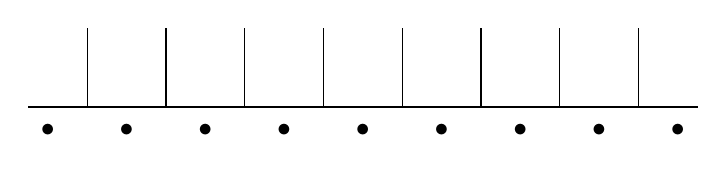
\begin{tikzpicture}
			\draw (-0.25,0) -- (8.25,0);
			\draw (0.5,0) -- (0.5,1);
			\draw (1.5,0) -- (1.5,1);
			\draw (2.5,0) -- (2.5,1);
			\draw (3.5,0) -- (3.5,1);
			\draw (4.5,0) -- (4.5,1);
			\draw (5.5,0) -- (5.5,1);
			\draw (6.5,0) -- (6.5,1);
			\draw (7.5,0) -- (7.5,1);
			\node at (0,-0.3) {$\bullet$};
			\node at (1,-0.3) {$\bullet$};
			\node at (2,-0.3) {$\bullet$};
			\node at (3,-0.3) {$\bullet$};
			\node at (4,-0.3) {$\bullet$};
			\node at (5,-0.3) {$\bullet$};
			\node at (6,-0.3) {$\bullet$};
			\node at (7,-0.3) {$\bullet$};
			\node at (8,-0.3) {$\bullet$};
		\end{tikzpicture},
	\end{figure}
\noindent
where the vertical lines are fixed and the bullets can either be $0$ or $1$ (according to the fusion rules), hence each bullet represents the space $\mathbb{C}^2$.
If we, for instance, only fuse $1$-particles to the chain, the value of the bullets is fixed by the fusion rules: When we fix the boundary labels (e.g., to $1$), the only possible labeling is
	\begin{figure}[H]
		\begin{tikzpicture}
			\draw (-0.25,0) -- (8.25,0);
			\draw (0.5,0) -- (0.5,1);
			\draw (1.5,0) -- (1.5,1);
			\draw (2.5,0) -- (2.5,1);
			\draw (3.5,0) -- (3.5,1);
			\draw (4.5,0) -- (4.5,1);
			\draw (5.5,0) -- (5.5,1);
			\draw (6.5,0) -- (6.5,1);
			\draw (7.5,0) -- (7.5,1);
			\node at (0.5,1.3) {$1$};
			\node at (1.5,1.3) {$1$};
			\node at (2.5,1.3) {$1$};
			\node at (3.5,1.3) {$1$};
			\node at (4.5,1.3) {$1$};
			\node at (5.5,1.3) {$1$};
			\node at (6.5,1.3) {$1$};
			\node at (7.5,1.3) {$1$};
			\node at (0,-0.3) {$1$};
			\node at (1,-0.3) {$0$};
			\node at (2,-0.3) {$1$};
			\node at (3,-0.3) {$0$};
			\node at (4,-0.3) {$1$};
			\node at (5,-0.3) {$0$};
			\node at (6,-0.3) {$1$};
			\node at (7,-0.3) {$0$};
			\node at (8,-0.3) {$1$};
		\end{tikzpicture}.
	\end{figure}
\noindent
Hence, we have a unique ground state and the only vertices occurring in this case are
	\begin{figure}[H]	
		\begin{tikzpicture}
			\draw (0,0) -- (1.5,0);
			\draw (0.75,0) -- (0.75,1);
			\node at (0,-0.3) {$0$};
			\node at (1.5,-0.3) {$1$};
			\node at (0.75,1.3) {$1$};
		\end{tikzpicture}
		\hspace{20pt}
		\begin{tikzpicture}
			\draw (0,0) -- (1.5,0);
			\draw (0.75,0) -- (0.75,1);
			\node at (0,-0.3) {$1$};
			\node at (1.5,-0.3) {$0$};
			\node at (0.75,1.3) {$1$};
		\end{tikzpicture}.
	\end{figure}
\noindent
Analogously, if we only allow $0$s to fuse to the chain, and the outer labels are fixed to $1$, the only possible labeling is 
	\begin{figure}[H]
		\begin{tikzpicture}
		\draw (-0.25,0) -- (8.25,0);
		\draw (0.5,0) -- (0.5,1);
		\draw (1.5,0) -- (1.5,1);
		\draw (2.5,0) -- (2.5,1);
		\draw (3.5,0) -- (3.5,1);
		\draw (4.5,0) -- (4.5,1);
		\draw (5.5,0) -- (5.5,1);
		\draw (6.5,0) -- (6.5,1);
		\draw (7.5,0) -- (7.5,1);
		\node at (0.5,1.3) {$0$};
		\node at (1.5,1.3) {$0$};
		\node at (2.5,1.3) {$0$};
		\node at (3.5,1.3) {$0$};
		\node at (4.5,1.3) {$0$};
		\node at (5.5,1.3) {$0$};
		\node at (6.5,1.3) {$0$};
		\node at (7.5,1.3) {$0$};
		\node at (0,-0.3) {$1$};
		\node at (1,-0.3) {$1$};
		\node at (2,-0.3) {$1$};
		\node at (3,-0.3) {$1$};
		\node at (4,-0.3) {$1$};
		\node at (5,-0.3) {$1$};
		\node at (6,-0.3) {$1$};
		\node at (7,-0.3) {$1$};
		\node at (8,-0.3) {$1$};
		\end{tikzpicture}.
	\end{figure}
	\noindent
If we had fixed the outer labels to $0$, all bullets would have to be $0$. Hence, the only vertices occurring in these cases are
	\begin{figure}[H]	
		\begin{tikzpicture}
		\draw (0,0) -- (1.5,0);
		\draw (0.75,0) -- (0.75,1);
		\node at (0,-0.3) {$0$};
		\node at (1.5,-0.3) {$0$};
		\node at (0.75,1.3) {$0$};
		\end{tikzpicture}
		\hspace{20pt}
		\begin{tikzpicture}
		\draw (0,0) -- (1.5,0);
		\draw (0.75,0) -- (0.75,1);
		\node at (0,-0.3) {$1$};
		\node at (1.5,-0.3) {$1$};
		\node at (0.75,1.3) {$0$};
		\end{tikzpicture}.
	\end{figure}
\noindent
This means that in the case of open boundary conditions, the chain has a \emph{unique ground state} once we fix the outer labels of the chain. The situation is different for periodic boundary conditions: since the only requirement here is that the label at site $n+1$ has to equal the label at site $1$, there are always two possibilities of labeling the chain. For instance, in the case of only fusing $1$s to the chain, the two possibilities are
	\begin{figure}[H]
		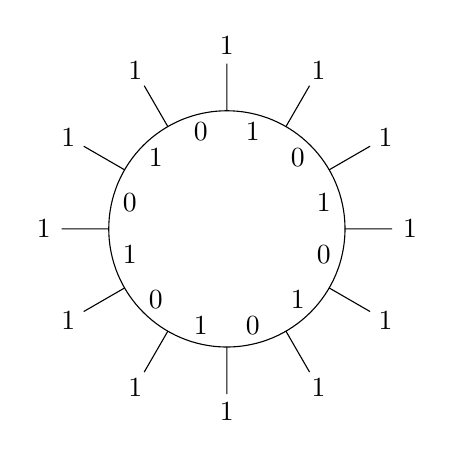
\begin{tikzpicture}[scale=1.5]
			\def\Radius{1cm}
			\draw (0,0) circle[radius=\Radius];
			\draw
			\foreach \a in {0, 30, ..., 330} {
				(\a:\Radius) -- (\a:1.4)
			};
			\foreach \a in {0, 30, ..., 330} {
				\node at (\a:1.55) {$1$};
			};
			\foreach \a in {45, 105, ..., 375} {
				\node at (\a:0.85) {$0$};
			};
			\foreach \a in {15, 75, ..., 315} {
				\node at (\a:0.85) {$1$};
			};
		\end{tikzpicture}
		\hspace{40pt}
		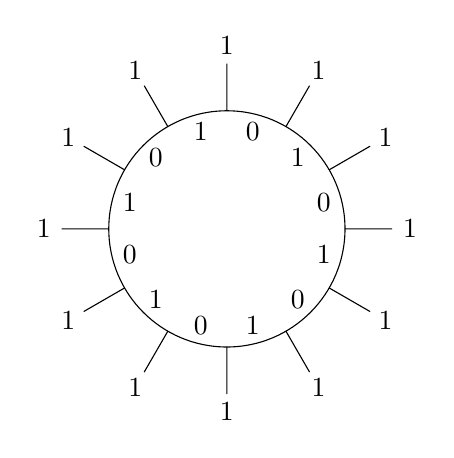
\begin{tikzpicture}[scale=1.5]
			\def\Radius{1cm}
			\draw (0,0) circle[radius=\Radius];
			\draw
			\foreach \a in {0, 30, ..., 330} {
				(\a:\Radius) -- (\a:1.4)
			};
			\foreach \a in {0, 30, ..., 330} {
				\node at (\a:1.55) {$1$};
			};
			\foreach \a in {45, 105, ..., 375} {
				\node at (\a:0.85) {$1$};
			};
			\foreach \a in {15, 75, ..., 315} {
				\node at (\a:0.85) {$0$};
			};
		\end{tikzpicture}.
	\end{figure}
\noindent
In case of fusing $0$ to the chain, we can either allow only $0$s or only $1$ as labels of the chain. Therefore, the chain with periodic boundary conditions has two ground states, hence it represents a qubit.

We will now introduce defects to this model, indicated by red lines that fuse to the chain, e.g.\ a chain with one defect would be
	\begin{figure}[H]
		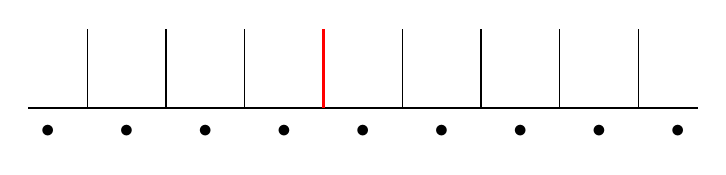
\begin{tikzpicture}
		\draw (-0.25,0) -- (8.25,0);
		\draw (0.5,0) -- (0.5,1);
		\draw (1.5,0) -- (1.5,1);
		\draw (2.5,0) -- (2.5,1);
		\draw[red,line width=0.4mm] (3.5,0) -- (3.5,1);
		\draw (4.5,0) -- (4.5,1);
		\draw (5.5,0) -- (5.5,1);
		\draw (6.5,0) -- (6.5,1);
		\draw (7.5,0) -- (7.5,1);
		\node at (0,-0.3) {$\bullet$};
		\node at (1,-0.3) {$\bullet$};
		\node at (2,-0.3) {$\bullet$};
		\node at (3,-0.3) {$\bullet$};
		\node at (4,-0.3) {$\bullet$};
		\node at (5,-0.3) {$\bullet$};
		\node at (6,-0.3) {$\bullet$};
		\node at (7,-0.3) {$\bullet$};
		\node at (8,-0.3) {$\bullet$};
		\end{tikzpicture}.
	\end{figure}
	\noindent
Since the chain is represented by a category, $\Vec(\Z/2\Z)$ in our example, the defect is a $\Vec(\Z/2\Z)$-$\Vec(\Z/2\Z)$ bimodule, i.e.\ we are fusing an object from the bimodule to the chain. Here, we will use the bimodule $F_1$ (see Subsection \ref{sec:VecZp-bimodules}) to introduce defects to the $\Vec(\Z/2\Z)$-chain. $F_1$ has only one object, so in general we omit writing labels for the bimodule object, but indicate by a red line when the object is from the bimodule. When it is useful to indicate the label, we denote it $*$.

The occurrence of one defect in a chain does not change the ground state of the system; The labels on the chain are still determined by the choice of labels on the boundary. This is different if we have more than one defect in the chain. For instance, for two defects the chain is
	\begin{figure}[H]
		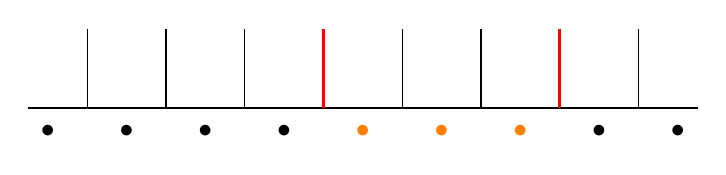
\begin{tikzpicture}
		\draw (-0.25,0) -- (8.25,0);
		\draw (0.5,0) -- (0.5,1);
		\draw (1.5,0) -- (1.5,1);
		\draw (2.5,0) -- (2.5,1);
		\draw[red,line width=0.4mm] (3.5,0) -- (3.5,1);
		\draw (4.5,0) -- (4.5,1);
		\draw (5.5,0) -- (5.5,1);
		\draw[red,line width=0.4mm] (6.5,0) -- (6.5,1);
		\draw (7.5,0) -- (7.5,1);
		\node at (0,-0.3) {$\bullet$};
		\node at (1,-0.3) {$\bullet$};
		\node at (2,-0.3) {$\bullet$};
		\node at (3,-0.3) {$\bullet$};
		\node at (4,-0.3) {{\color{orange}$\bullet$}};
		\node at (5,-0.3) {{\color{orange}$\bullet$}};
		\node at (6,-0.3) {{\color{orange}$\bullet$}};
		\node at (7,-0.3) {$\bullet$};
		\node at (8,-0.3) {$\bullet$};
		\end{tikzpicture},
	\end{figure}
\noindent
where the colour of the orange bullets is not determined by the labels on the boundary of the chain. Hence, we get an additional qubit. In general, the number of additional qubits in the chain is $\#\mathrm{defects}-1$. This can be done analogously for the chain with periodic boundary conditions, the only difference is that in this case, we already have one qubit when there is no defect.

We could also allow the bimodule object to live on the horizontal lines of the chain. In particular,
We now want to build a chain out of $\Vec(\Z/2\Z)$ and the bimodule $F_1$ in the following way: consider the chain
\begin{figure}[H]
	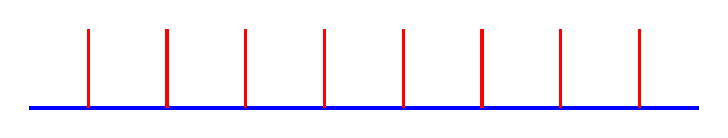
\begin{tikzpicture}
	\draw[blue,line width=0.4mm] (-0.25,0) -- (8.25,0);
	\draw[red,line width=0.4mm] (0.5,0) -- (0.5,1);
	\draw[red,line width=0.4mm] (1.5,0) -- (1.5,1);
	\draw[red,line width=0.4mm] (2.5,0) -- (2.5,1);
	\draw[red,line width=0.4mm] (3.5,0) -- (3.5,1);
	\draw[red,line width=0.4mm] (4.5,0) -- (4.5,1);
	\draw[red,line width=0.4mm] (5.5,0) -- (5.5,1);
	\draw[red,line width=0.4mm] (6.5,0) -- (6.5,1);
	\draw[red,line width=0.4mm] (7.5,0) -- (7.5,1);
	\end{tikzpicture},
\end{figure}
\noindent
where
\begin{equation}\label{eq:configs}

\begin{tikzpicture}[scale=1,baseline=(current bounding box.center)]
\draw[blue,line width=0.4mm] (0,0) -- (1,0);
\end{tikzpicture}=
\begin{tikzpicture}[scale=1,baseline=(current bounding box.center)]
\draw[black] (0,0) -- (1,0);
\end{tikzpicture}\oplus

\begin{tikzpicture}[scale=1,baseline=(current bounding box.center)]
\draw[red,line width=0.4mm] (0,0) -- (1,0);
\end{tikzpicture},
\end{equation}
which means that it is either an object from the category ($0$ or $1$) or an object from the bimodule (which can only be $*$), i.e., $\mathbb{C}^2\oplus\mathbb{C}\cong\mathbb{C}^3$. Valid configurations then look like
\begin{figure}[H]
	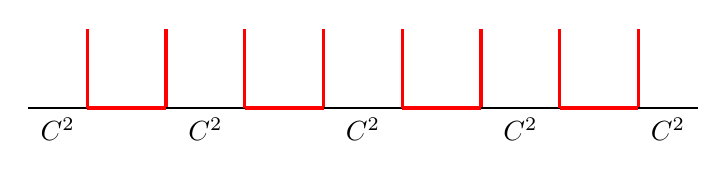
\begin{tikzpicture}
	\draw[black] (-0.25,0) to node [below] {$\mathbb{C}^2$} (0.5,0);
	\draw[red,line width=0.4mm] (0.5,0) -- (0.5,1);
	\draw[red,line width=0.4mm] (0.5,0) -- (1.5,0);
	\draw[red,line width=0.4mm] (1.5,0) -- (1.5,1);
	\draw[black] (1.5,0) to node [below] {$\mathbb{C}^2$} (2.5,0);
	\draw[red,line width=0.4mm] (2.5,0) -- (2.5,1);
	\draw[red,line width=0.4mm] (2.5,0) -- (3.5,0);
	\draw[red,line width=0.4mm] (3.5,0) -- (3.5,1);
	\draw[black] (3.5,0) to node [below] {$\mathbb{C}^2$} (4.5,0);
	\draw[red,line width=0.4mm] (4.5,0) -- (4.5,1);
	\draw[red,line width=0.4mm] (4.5,0) -- (5.5,0);
	\draw[red,line width=0.4mm] (5.5,0) -- (5.5,1);
	\draw[black] (5.5,0) to node [below] {$\mathbb{C}^2$} (6.5,0);
	\draw[red,line width=0.4mm] (6.5,0) -- (6.5,1);
	\draw[red,line width=0.4mm] (6.5,0) -- (7.5,0);
	\draw[red,line width=0.4mm] (7.5,0) -- (7.5,1);
	\draw[black] (7.5,0) to node [below] {$\mathbb{C}^2$} (8.25,0);
	\end{tikzpicture}
\end{figure}
\noindent
so we have a non-trivial Hilbert space. Our goal is to construct a Hamiltonian for this chain that is similar to the golden chain Hamiltonian in \cite{Feiguin2007}, where a chain model for the Fibonacci category was constructed which energetically favoured fusing to the vacuum. For our chain model, this means that it is energetically favoured to fuse to the $0$ object of $\Vec(\Z/2\Z)$. Hence, the Hamiltonian is of the form
\begin{equation}
H=-\sum \frac{1}{\sqrt{2}}
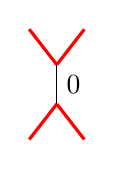
\begin{tikzpicture}[scale=0.5,baseline=(current bounding box.center)]
\draw[red,line width=0.4mm] (0,0) -- (-0.7,0.9);
\draw[red,line width=0.4mm] (0,0) -- (0.7,0.9);
\draw (0,0) to node[right] {$0$} (0,-1);
\draw[red,line width=0.4mm] (0,-1) -- (-0.7,-1.9);
\draw[red,line width=0.4mm] (0,-1) -- (0.7,-1.9);
%			\node at (0.8,1.1) {$*$};
%			\node at (-0.8,1.1) {$*$};
%			\node at (0.8,-2.1) {$*$};
%			\node at (-0.8,-2.1) {$*$};
\end{tikzpicture},\label{VecZ2Hamiltonian}
\end{equation}
where the sum goes over all sites of the chain. This Hamiltonian involves the vertex
\begin{figure}[H]	
	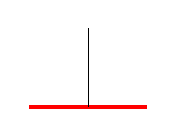
\begin{tikzpicture}
	\draw[red,line width=0.4mm] (0,0) -- (1.5,0);
	\draw[black] (0.75,0) -- (0.75,1);
	\end{tikzpicture}.
\end{figure}
\noindent
Since this vertex is neither defined in the category $\Vec(\Z/2\Z)$ nor in the bimodule $F_1$, we need to construct it. More precisely, for each choice of labels we need a basis for the corresponding morphism space. 
%For now, we will restrict to the case that only objects of the category are allowed to be on horizontal lines, but we will come back to other possibilities later. Although we will not need this specific vertex in the final chain we are going to construct, we go through its computation in detail to explain how these vertices can be constructed in general. 
We do the construction of the required vertex step-by-step in Section~\ref{Ising} using ideas from tube algebras. Therefore, we familiarize the reader with these concepts first.

\section{Background}\label{S:defs}
In this section, we provide all the definitions and notation in the vein of category theory that are used throughout the subsequent computations. We do not give exhaustive details and explanations whenever it is not necessary for this work but refer to the literature where those can be found.

% This line sets the project root file.
% !TEX root = Notes_Gauging_Defects.tex
% !TEX spellcheck = en_US

\subsection{Fusion categories}

We briefly recall the definition of a fusion category, omitting many details. A full definition can be found in Chapter 4 of \cite{Etingof2015}.
\begin{definition}[Fusion category]
	A tensor category $\cat$ is a $\mathbb{C}$-linear category $\cat$ with a functor $\otimes:\cat\times\cat\to\cat$, a natural isomorphism $(-\otimes-)\otimes-\cong-\otimes(-\otimes-)$ called the associator, and a unit object $1$.
	These data must satisfy coherence equations such as the pentagon equations, that can be found in Section 2.1 of \cite{Etingof2015}.
	
	A \emph{fusion category} is a rigid\footnote{We refer the reader to \cite{Etingof2015} for details.} semisimple tensor category with finitely many isomorphism classes of simple objects and $\End(1)\cong \mathbb{C}$.
	
	It is convenient to describe a fusion category $\cat$ using \emph{skeletal data}. This approach is standard in the (physics) literature, and amounts to picking representatives for each isomorphism class of simple object. The full fusion category can be canonically reconstructed from the skeletal data \cite{BBJSkeletal}. A \emph{skeletal fusion category} consists of:
	\begin{itemize}
		\item A finite set of simple objects $L=\{1,a,b,c,\ldots\}$ , where $1$ is the distinguished unit object.
		\item For each triple $(a,b;c)$ a finite dimensional Hilbert space $C(a\otimes b,c)$ represented as a trivalent vertex
		\begin{equation}
		\begin{tikzpicture}[scale=0.8,baseline=(current bounding box.center)]
		\draw (-.707,-.707)--(0,0) node[pos=-.25] {$a$};
		\draw (.707,-.707)--(0,0) node[pos=-.25] {$b$};
		\draw (0,0)--(0,1) node[pos=1.25] {$c$};
		\end{tikzpicture}.
		\end{equation} 
		\item An associator. If a basis is picked for each $C(-\otimes -,-)$ (here we assume these are all 1 dimensional for simplicity), the associator can be represented as a tensor $F$
		\begin{equation}
		\begin{tikzpicture}[scale=0.8,baseline=(current bounding box.center)]
		\draw (0,0)--(0,1) node[pos=1.25] {$d$};
		\draw (0,0)--(1.41,-1.41) node[pos=1.15] {$c$};
		\draw (0,0)--(-.707,-.707) node [pos=.5,above left] {$e$};
		\draw (-.707,-.707)--(-1.41,-1.41)node[pos=1.25] {$a$};
		\draw (-.707,-.707)--(0,-1.41)node[pos=1.25] {$b$};
		\end{tikzpicture}
		=\sum_{f\in L}\left(F_{abc}^{d}\right)_{e,f}
		\begin{tikzpicture}[scale=0.8,baseline=(current bounding box.center)]
		\draw (0,0)--(0,1) node[pos=1.25] {$d$};
		\draw (.707,-.707)--(1.41,-1.41) node[pos=1.25] {$c$};
		\draw (0,0)--(.707,-.707) node [pos=.5,above right] {$f$};
		\draw (0,0)--(-1.41,-1.41)node[pos=1.15] {$a$};
		\draw (.707,-.707)--(0,-1.41)node[pos=1.25] {$b$};
		\end{tikzpicture}.\label{eqn:Fsymbdef}
		\end{equation} 
		The tensors are often called the $F$-symbols.
	\end{itemize}
\end{definition}

\begin{example}[$\Vec(G)$]\label{example:vecG}
	Let $G$ be a finite group. The category $\Vec(G)$ is the category of $G$-graded vector spaces. The skeletal description is very simple. The set of simples is $G$ as a set, with the group identity becoming the unit. The vector spaces are 0 dimensional except $C(g\otimes h, gh)$ which is 1 dimensional for all $g,h$. The $F$-symbols are $+1$ when the diagrams in \eqref{eqn:Fsymbdef} are nonzero.
\end{example}
% This line sets the project root file.
% !TEX root = Notes_Gauging_Defects.tex
% !TEX spellcheck = en_US

\subsection{Bimodules}

\begin{definition}
	Let $\mathcal{C}$ be a fusion category. A \textbf{left module category} over $\mathcal{C}$ is a semi-simple category $\mathcal{M}$ equipped with a left $\mathcal{C}$-\emph{action}, i.e.\ a functor $\triangleright:\mathcal{C}\times\mathcal{M}\to\mathcal{M}$ and a natural isomorphism 
		\begin{equation}
			a\triangleright(b\triangleright m)\cong(a\otimes b)\triangleright m
		\end{equation}
	which satisfies some coherence conditions that can be found in Sec.~7.1 of \cite{Etingof2015}. If we choose bases for all the vector spaces $\mathcal{M}(a\triangleright m,n)$, this associator can be written in terms of a tensor $L$ using string diagrams
		\begin{equation}
			\begin{tikzpicture}[scale=0.9,baseline=(current bounding box.center)]
			\node[bwred](m) at (0,0) {$m$};
			\node(b) at (-1,0) {$b$};
			\node(a) at (-2,0) {$a$};
			\node[bwred](abm) at (0,3) {$n$};
			\draw[bwred,line width=0.4mm] (m) to node[right] {$p$} (abm);
			\draw (b) to [bend left] (0,1);
			\draw (a) to [bend left] (0,2);
			\end{tikzpicture}\ =\sum_q \left(L^n_{abm}\right)_{p,q}
			\begin{tikzpicture}[scale=0.9,baseline=(current bounding box.center)]
			\node[bwred](m) at (0,0) {$m$};
			\node(b) at (-1,0) {$b$};
			\node(a) at (-2,0) {$a$};
			\node[bwred](abm) at (0,3) {$n$};
			\node(ab) at (-1.2,1.8) {$q$};
			\draw[bwred,line width=0.4mm] (m) to (abm);
			\draw (b) to [bend right] (-1.5,1.1);
			\draw (a) to [bend left] (0,2);
			\end{tikzpicture},\label{eqn:L}
		\end{equation}
	where we have marked the objects of the module category in red. One can define a \textbf{right module category} over $\mathcal{C}$ in a similar way: Here, we have a semi-simple category $\mathcal{M}$ with a functor $\triangleleft:\mathcal{M}\times\mathcal{C}\to\mathcal{M}$ and a natural isomorphism
		\begin{equation}
			(m\triangleleft a)\triangleleft b\cong m\triangleleft(a\otimes b)
		\end{equation}
	(satisfying some coherence conditions), which we can represent by a tensor $R$:
		\begin{equation}
			\begin{tikzpicture}[scale=0.9,baseline=(current bounding box.center)]
			\node[bwred](m) at (0,0) {$m$};
			\node(b) at (1,0) {$a$};
			\node(a) at (2,0) {$b$};
			\node[bwred](abm) at (0,3) {$n$};
			\draw[bwred,line width=0.4mm] (m) to node [left] {$p$} (abm);
			\draw (b) to [bend right] (0,1);
			\draw (a) to [bend right] (0,2);
			\end{tikzpicture}\ =\sum_q\left(R^n_{mab}\right)_{p,q}
			\begin{tikzpicture}[scale=0.9,baseline=(current bounding box.center)]
			\node[bwred](m) at (0,0) {$m$};
			\node(b) at (1,0) {$a$};
			\node(a) at (2,0) {$b$};
			\node[bwred](abm) at (0,3) {$n$};
			\node(ab) at (1.2,1.8) {$q$};
			\draw[bwred,line width=0.4mm] (m) to (abm);
			\draw (b) to [bend left] (1.5,1.1);
			\draw (a) to [bend right] (0,2);
			\end{tikzpicture}.\label{eqn:R}
		\end{equation}
\end{definition}

\begin{definition}
	Let $\mathcal{C}, \mathcal{D}$ be fusion categories. A $(\mathcal{C},\mathcal{D})$-\textbf{bimodule category} (also written $\mathcal{C}\curvearrowright\mathcal{M}\curvearrowleft\mathcal{D}$) is a semi-simple category $\mathcal{M}$ that has left $\mathcal{C}$-module and right $\mathcal{D}$-module category structures, i.e.\ there are natural isomorphisms 
		\begin{align}
			a\triangleright(b\triangleright m)&\cong(a\otimes b)\triangleright m\\ 
			(m\triangleleft a)\triangleleft b&\cong m\triangleleft(a\otimes b)
		\end{align}
	that satisfy certain coherence conditions between $L$ and $R$. Additionally, there is a natural isomorphism 
		\begin{equation}
			a\triangleright(m\triangleleft b)\cong (a\triangleright m)\triangleleft b.
		\end{equation}
	As above, after choosing bases for the morphism spaces, this can be represented in terms of string diagrams with a tensor $C$:
		\begin{equation}
			\begin{tikzpicture}[scale=0.9,baseline=(current bounding box.center)]
			\node[bwred](m) at (0,0) {$m$};
			\node(a) at (-1,0) {$a$};
			\node(b) at (1,0) {$b$};
			\node[bwred](abm) at (0,3) {$n$};
			\draw[bwred,line width=0.4mm] (m) to node [left] {$p$} (abm);
			\draw (a) to [bend left] (0,1);
			\draw (b) to [bend right] (0,2);
			\end{tikzpicture}\ =\sum_q\left(C^n_{amb}\right)_{pq}
			\begin{tikzpicture}[scale=0.9,baseline=(current bounding box.center)]
			\node[bwred](m) at (0,0) {$m$};
			\node(a) at (-1,0) {$a$};
			\node(b) at (1,0) {$b$};
			\node[bwred](abm) at (0,3) {$n$};
			\draw[bwred,line width=0.4mm] (m) to node [right] {$q$} (abm);
			\draw (b) to [bend right] (0,1);
			\draw (a) to [bend left] (0,2);
			\end{tikzpicture}.
		\end{equation}
\end{definition}

% This line sets the project root file.
% !TEX root = Notes_Gauging_Defects.tex
% !TEX spellcheck = en_US

\subsection{Example: $\Vec(\Z/p\Z)$ bimodules}\label{sec:VecZp-bimodules}

We will now list all the $\Vec(\Z/p\Z)$-$\Vec(\Z/p\Z)$ bimodules since we are going to need them in Subsection \ref{subsec:VecZ2}. This data is mostly taken from \cite{BBJ19}, and the names assigned to the bimodules are taken from there. Each bimodule $\mathcal{M}$ is labeled by a conjugacy class of subgroups $H\subseteq\Z/p\Z\times\Z/p\Z$ and a $2-$cocycle $\omega\in H^2(H,U(1))$ (see \cite{Etingof2015}). The objects of $\mathcal{M}$ are labeled by cosets of $H$. In general, there are four non-invertible bimodules: 
	\begin{enumerate}
		\item The trivial bimodule $T$, which is coming from the subgroup $\{(0,0)\}$. It has $p^2$ simple objects, which are labeled by the cosets $\{(g,h)\}$ of the group, i.e.\ a simple object in $T$ is $(g,h)$. The left and right action is given as follows
			\begin{equation}
				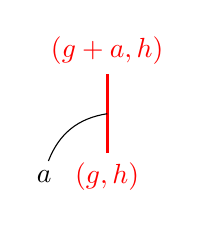
\begin{tikzpicture}[scale=0.8,baseline=(current bounding box.center)]
				\node[red](m) at (0,0) {$(g,h)$};
				\node(b) at (-1,0) {$a$};
				\node[red](abm) at (0,2) {$(g+a,h)$};
				\draw[red,line width=0.4mm] (m)-- (abm);
				\draw (b) to [bend left] (0,1);
				\end{tikzpicture}\hspace{20pt}
				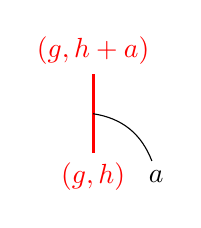
\begin{tikzpicture}[scale=0.8,baseline=(current bounding box.center)]
				\node[red](m) at (0,0) {$(g,h)$};
				\node(b) at (1,0) {$a$};
				\node[red](abm) at (0,2) {$(g,h+a)$};
				\draw[red,line width=0.4mm] (m)-- (abm);
				\draw (b) to [bend right] (0,1);
				\end{tikzpicture}
			\end{equation}
		\noindent
		and the associator for this bimodule is trivial:
			\begin{equation}
				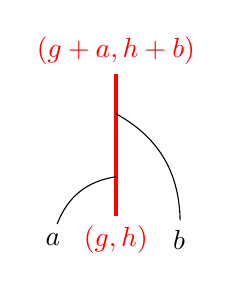
\begin{tikzpicture}[scale=0.8,baseline=(current bounding box.center)]
				\node[red](m) at (0,0) {$(g,h)$};
				\node(a) at (-1,0) {$a$};
				\node(b) at (1,0) {$b$};
				\node[red](abm) at (0,3) {$(g+a,h+b)$};
				\draw[red,line width=0.4mm] (m) -- (abm);
				\draw (a) to [bend left] (0,1);
				\draw (b) to [bend right] (0,2);
				\end{tikzpicture}\ =
				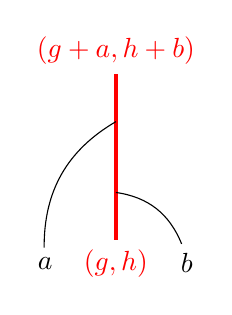
\begin{tikzpicture}[scale=0.9,baseline=(current bounding box.center)]
				\node[red](m) at (0,0) {$(g,h)$};
				\node(a) at (-1,0) {$a$};
				\node(b) at (1,0) {$b$};
				\node[red](abm) at (0,3) {$(g+a,h+b)$};
				\draw[red,line width=0.4mm] (m) -- (abm);
				\draw (b) to [bend right] (0,1);
				\draw (a) to [bend left] (0,2);
				\end{tikzpicture}.
			\end{equation}
		\item The bimodule $L$ from the subgroup $H=\langle(1,0)\rangle\cong \Z/p\Z$, which has $p$ simple objects. The labels are given by the cosets $\{(h,g)|h\in\Z/p\Z\}$, hence the label for a simple object in $L$ is $g$. Left and right action are given by 
			\begin{equation}
				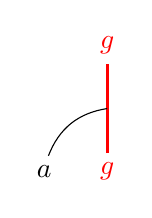
\begin{tikzpicture}[scale=0.8,baseline=(current bounding box.center)]
				\node[red](m) at (0,0) {$g$};
				\node(b) at (-1,0) {$a$};
				\node[red](abm) at (0,2) {$g$};
				\draw[red,line width=0.4mm] (m)-- (abm);
				\draw (b) to [bend left] (0,1);
				\end{tikzpicture}\hspace{20pt}
				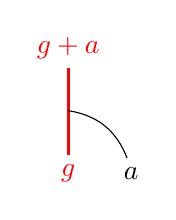
\begin{tikzpicture}[scale=0.8,baseline=(current bounding box.center)]
				\node[red](m) at (0,0) {$g$};
				\node(b) at (1,0) {$a$};
				\node[red](abm) at (0,2) {$g+a$};
				\draw[red,line width=0.4mm] (m)-- (abm);
				\draw (b) to [bend right] (0,1);
				\end{tikzpicture}
			\end{equation}
		and the associator is trivial.
		\item The bimodule $R$ from the subgroup $H=\langle(0,1)\rangle\cong \Z/p\Z$. This bimodule is basically the same as $L$, but in all operations left and right are flipped.
		\item $F_0$, the bimodule from the subgroup $\langle(0,1),(1,0)\rangle\cong\Z/p\Z\times\Z/p\Z$, which has only one object that is denoted $*$. Left and right actions are
			\begin{equation}
				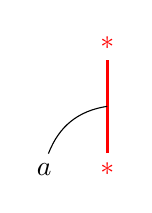
\begin{tikzpicture}[scale=0.8,baseline=(current bounding box.center)]
				\node[red](m) at (0,0) {$*$};
				\node(b) at (-1,0) {$a$};
				\node[red](abm) at (0,2) {$*$};
				\draw[red,line width=0.4mm] (m)-- (abm);
				\draw (b) to [bend left] (0,1);
				\end{tikzpicture}\hspace{20pt}
				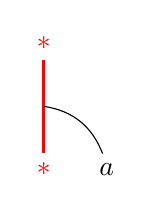
\begin{tikzpicture}[scale=0.8,baseline=(current bounding box.center)]
				\node[red](m) at (0,0) {$*$};
				\node(b) at (1,0) {$a$};
				\node[red](abm) at (0,2) {$*$};
				\draw[red,line width=0.4mm] (m)-- (abm);
				\draw (b) to [bend right] (0,1);
				\end{tikzpicture}
			\end{equation}
		\noindent
		and the associator is trivial.
	\end{enumerate}
Furthermore, there are several invertible bimodules:
	\begin{enumerate}
		\item The bimodule $X_k$, coming from the subgroup $\{(-k,1)\}\cong\Z/p\Z$ with $p$ simple objects. The cosets of this group are $\{n(-k,1)+(h,0)|n\in\Z/p\Z\}$, hence the object labels are $h$. Left and right action is given by 
			\begin{equation}
				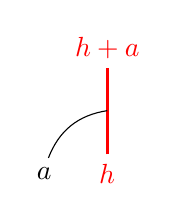
\begin{tikzpicture}[scale=0.8,baseline=(current bounding box.center)]
				\node[red](m) at (0,0) {$h$};
				\node(b) at (-1,0) {$a$};
				\node[red](abm) at (0,2) {$h+a$};
				\draw[red,line width=0.4mm] (m)-- (abm);
				\draw (b) to [bend left] (0,1);
				\end{tikzpicture}\hspace{20pt}
				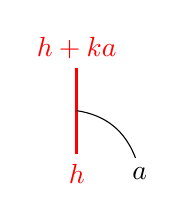
\begin{tikzpicture}[scale=0.8,baseline=(current bounding box.center)]
				\node[red](m) at (0,0) {$h$};
				\node(b) at (1,0) {$a$};
				\node[red](abm) at (0,2) {$h+ka$};
				\draw[red,line width=0.4mm] (m)-- (abm);
				\draw (b) to [bend right] (0,1);
				\end{tikzpicture}
			\end{equation}
		\noindent
		and the associator is again trivial.
		\item The bimodule $F_q$, with $q\in H^2(\Z/p\Z,U(1))\cong\Z/q\Z$. As $F_0$, it comes from the subgroup $\langle(0,1),(1,0)\rangle$ and has only one object denoted $*$. Also, left and right action are defined in the same way as they are in $F_0$, but now the associator is non-trivial:
			\begin{equation}
				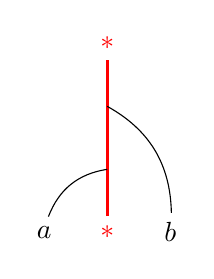
\begin{tikzpicture}[scale=0.8,baseline=(current bounding box.center)]
				\node[red](m) at (0,0) {$*$};
				\node(a) at (-1,0) {$a$};
				\node(b) at (1,0) {$b$};
				\node[red](abm) at (0,3) {$*$};
				\draw[red,line width=0.4mm] (m) -- (abm);
				\draw (a) to [bend left] (0,1);
				\draw (b) to [bend right] (0,2);
				\end{tikzpicture}\ =e^{\frac{2\pi i}{p}qab}
				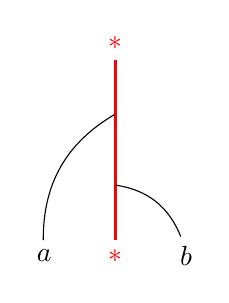
\begin{tikzpicture}[scale=0.9,baseline=(current bounding box.center)]
				\node[red](m) at (0,0) {$*$};
				\node(a) at (-1,0) {$a$};
				\node(b) at (1,0) {$b$};
				\node[red](abm) at (0,3) {$*$};
				\draw[red,line width=0.4mm] (m) -- (abm);
				\draw (b) to [bend right] (0,1);
				\draw (a) to [bend left] (0,2);
				\end{tikzpicture}.
			\end{equation}
		We are especially interested in the $\Vec(\Z/2\Z)$-$\Vec(\Z/2\Z)$ bimodule $F_1$ which we use to introduce defects to a $\Vec(\Z/2\Z)$ spin chain. In this case the associator is given by
			\begin{equation}
				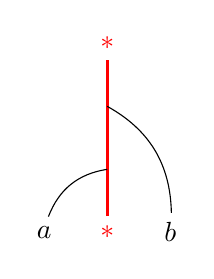
\begin{tikzpicture}[scale=0.8,baseline=(current bounding box.center)]
				\node[red](m) at (0,0) {$*$};
				\node(a) at (-1,0) {$a$};
				\node(b) at (1,0) {$b$};
				\node[red](abm) at (0,3) {$*$};
				\draw[red,line width=0.4mm] (m) -- (abm);
				\draw (a) to [bend left] (0,1);
				\draw (b) to [bend right] (0,2);
				\end{tikzpicture}\ =(-1)^{ab}
				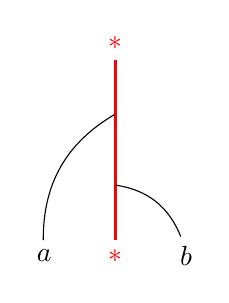
\begin{tikzpicture}[scale=0.9,baseline=(current bounding box.center)]
				\node[red](m) at (0,0) {$*$};
				\node(a) at (-1,0) {$a$};
				\node(b) at (1,0) {$b$};
				\node[red](abm) at (0,3) {$*$};
				\draw[red,line width=0.4mm] (m) -- (abm);
				\draw (b) to [bend right] (0,1);
				\draw (a) to [bend left] (0,2);
				\end{tikzpicture}.\label{eqn:F1}
			\end{equation}
	\end{enumerate}


% This line sets the project root file.
% !TEX root = Notes_Gauging_Defects.tex
% !TEX spellcheck = en_US

\subsection{Bimodule tensor products}\label{sec:bimodtensor}

To extend a category $\cat$ to include bimodule objects, we need to introduce `bimodule trivalent vertices'. To construct these, we need a product on bimodules. 

\begin{definition}[Relative tensor product]
	Given bimodules $\mathcal{A}\curvearrowright\mathcal{M}\curvearrowleft\mathcal{B}\curvearrowright{\mathcal{N}}\curvearrowleft\mathcal{C}$, the \emph{relative tensor product} $\mathcal{M}\otimes_\mathcal{B}\mathcal{N}$ has objects $(m,n)\in \mathcal{M}\otimes\mathcal{N}$, along with isomorphisms $\beta:(m\triangleleft b,n)\cong(m,b\triangleright n)$. The isomorphisms should be compatible with the module structure, for example
	\begin{align}
	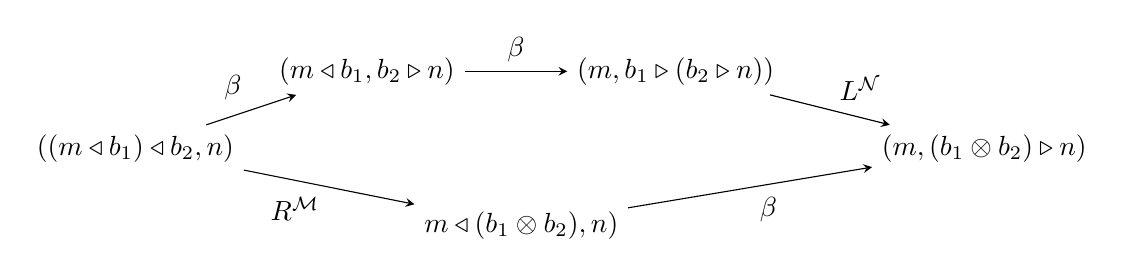
\begin{tikzpicture}[scale=.98,baseline=(current bounding box.center)]
	\node (A) at (-1,0) {$((m\triangleleft b_1)\triangleleft b_2,n)$};
	\node (B) at (2,1) {$(m\triangleleft b_1,b_2\triangleright n)$};
	\node (C) at (6,1) {$(m,b_1\triangleright(b_2\triangleright n))$};
	\node (D) at (10,0) {$(m,(b_1\otimes b_2)\triangleright n)$};
	\node (E) at (4,-1) {$m\triangleleft (b_1\otimes b_2), n)$};
	\draw [-stealth,above left] (A)--(B) node [pos=.5] {$\beta$};
	\draw [-stealth,above] (B)--(C) node [pos=.5] {$\beta$};
	\draw [-stealth,above right] (C)--(D) node [pos=.5] {$L^\mathcal{N}$};
	\draw [-stealth,below left] (A)--(E) node [pos=.5] {$R^{\mathcal{M}}$};
	\draw [-stealth,below right] (E)--(D) node [pos=.5] {$\beta$};
	\end{tikzpicture},
	\end{align}
	commutes. Here, $L^\mathcal{N}$ denotes the associator for the left action in $\mathcal{N}$ and $R^\mathcal{M}$ denotes the associator for the right action in $\mathcal{M}$. Morphisms in $\mathcal{M}\otimes_\mathcal{B}\mathcal{N}$ are morphisms in $\mathcal{M}\otimes\mathcal{N}$ that are compatible with $\beta$. $\mathcal{M}\otimes_\mathcal{B}\mathcal{N}$ is an $\mathcal{A}$-$\mathcal{C}$ bimodule, and can be decomposed into simple bimodules $\mathcal{P}$  $$\mathcal{M}\otimes_\mathcal{B}\mathcal{N}\cong\oplus_\mathcal{P}N_{\mathcal{M},\mathcal{N}}^\mathcal{P}\mathcal{P},$$
	where the $N_{\mathcal{M,N}}^\mathcal{P}$ are the corresponding coefficients in the decomposition. A complete definition can be found in \cite{DSPS14}.
\end{definition}

If a given bimodule $\mathcal{P}$ occurs in the decomposition of $\mathcal{M}\otimes_\mathcal{B}\mathcal{N}$, it is natural to introduce bimodule trivalent vertices of the form
\begin{align}
\begin{tikzpicture}[baseline=(current bounding box.center)]
\node (A) at (-.707,-.707) {$m\in\mathcal{M}$};
\node (B) at (.707,-.707) {$n\in\mathcal{N}$};
\node (C) at (0,1) {$p\in\mathcal{P}$};
\draw[violet,line width=0.4mm](A)--(0,0);
\draw[brown,line width=0.4mm](B)--(0,0);
\draw[nicegreen,line width=0.4mm](0,0)--(C);
\end{tikzpicture}.
\end{align}
This is the essence of the `inflation trick' developed in \cite{BBJ18,BB19a,BB19b}. We refer the interested reader to these references for more details. 
% This line sets the project root file.
% !TEX root = Notes_Gauging_Defects.tex
% !TEX spellcheck = en_US

\subsection{Definition of the annular category}

%Let $\cat$ be a fusion category with objects $\mathrm{obj}(\cat)=\{X,Y,Z,...\}$, morphisms $\mathrm{hom}(X,Y)=\left\{f:X\rightarrow Y\vert X,Y\in\mathrm{obj}(\cat)\right\}$ and simple objects $\mathrm{Irr}(\cat)=\{A,B,C,...\}$. We denote an isomorphism class of objects in $\cat$ by $[U]$ and fix a representative $U_C$ in each isomorphism class, i.e. identify each isomorphism class with a simple object $C\in \mathrm{Irr}(\cat)$. The tube algebra $\tub$ is an algebra associated with $\cat$ given by the following construction
%\begin{align}
%	\tub&=\bigoplus_{A,B\in\mathrm{Irr}(\cat)}\,\tub_{BA}\\
%	\tub_{BA}&=\bigoplus_{C\in\mathrm{Irr}(\cat)}\, \mathrm{hom}(U_C\otimes U_A,U_B\otimes U_C).
%\end{align}
%\noindent
%The objects in $\tub$ are the same as the objects in $\cat$ where the morphisms are given by
%\begin{equation}
%	\mathrm{hom}(A,B)=X\otimes A\rightarrow B\otimes X.
%\end{equation}
%
The first step in our gauging process for a collection of bimodules $\{\mathcal{M}_i\}$ is to extend the fusion category $\cat$ to include the objects in $\mathcal{M}_i$. From Section~\ref{sec:bimodtensor}, we have fusion rules for bimodules $\mathcal{M}\otimes\mathcal{N}=\oplus\mathcal{P}$. We utilize the \emph{annular category} to obtain trivalent vertices for these processes. 

\begin{definition}[3-string annular category]
	Let $\mathcal{A},\mathcal{B}$ and $\mathcal{C}$ be fusion categories, and $\mathcal{A}\curvearrowright\mathcal{M}\curvearrowleft\mathcal{B}\curvearrowright\mathcal{N}\curvearrowleft\mathcal{C}$ and $\mathcal{A}\curvearrowright\mathcal{P}\curvearrowleft\mathcal{C}$ bimodule categories. The 3-string annular category $\ann_{\mathcal{M},\mathcal{N};\mathcal{P}}(\mathcal{A},\mathcal{B},\mathcal{C})$ is defined as follows:
	The simple objects are triples $(m,n;p)\in\mathcal{M}\times\mathcal{N}\times\mathcal{P}$. A basis for the morphism space $(m,n;p)\to (m^\prime,n^\prime;p^\prime)$ is given by valid diagrams on the annulus (up to isotopy and local relations)
	\begin{equation}
		\begin{tikzpicture}[scale=1.2,baseline=(current bounding box.center)]
		\draw (0,0) circle (0.5cm);
		\draw (0,0) circle (1.6cm);
		\draw[brown,line width=0.4mm] (-60:0.5) -- (-60:1.6);
		\draw[violet,line width=0.4mm] (-120:0.5) -- (-120:1.6);
		\draw ([shift=(-60:1cm)]0,0) arc (-60:90:1cm);
		\draw ([shift=(-120:1.15cm)]0,0) arc (-120:-60:1.15cm);
		\draw ([shift=(240:0.85cm)]0,0) arc (240:90:0.85cm);
		\draw[nicegreen,line width=0.4mm] (90:0.5) -- (90:1.6);
		\node at (90:.3cm){$p$};\node at (90:1.8cm){$p'$};
		\node at (-60:.3cm){$n$};\node at (-60:1.8cm){$n'$};
		\node at (-120:.3cm){$m$};\node at (-120:1.8cm){$m'$};
		\node at (-1,0.3) {$a$};
		\node at (1.15,0.3) {$c$};
		\node at (0,-1.3) {$b$};
		\end{tikzpicture}\ .\label{eqn:basisann}
	\end{equation}
%	\begin{equation}
%	\begin{tikzpicture}[scale=0.8,baseline=(current bounding box.center)]
%	\def \rinner{.75};
%	\def \router{2};
%%	\node[red](m) at (0,0) {$*$};
%%	\node(a) at (-1,0) {$a$};
%%	\node(b) at (1,0) {$b$};
%%	\node[red](abm) at (0,3) {$*$};
%%	\draw[red] (m) -- (abm);
%%	\draw (a) to [bend left] (0,1);
%%	\draw (b) to [bend right] (0,2);
%	\draw (0,0) circle (\rinner);
%	\node[] at (90:\rinner-.25) {$p$};
%	\node[] at (240:\rinner-.25) {$m$};
%	\node[] at (300:\rinner-.25) {$n$};
%	\draw (0,0) circle (\router);
%	\node[] at (90:\router+.25) {$p^\prime$};
%	\node[] at (240:\router+.3) {$m^\prime$};
%	\node[] at (300:\router+.3) {$n^\prime$};
%	\draw[blue] (90:\rinner)--(90:\router);
%	\draw[red] (240:\rinner)--(240:\router);
%	\draw[nicegreen] (300:\rinner)--(300:\router);
%	\draw (240:1) to[out=90,in=240] (165:1) to [out=60,in=240] (90:1.25);
%	\draw (300:1) to[out=90,in=300] (15:1) to [out=120,in=300] (90:1.5);
%	\draw (240:1.75) to[out=40,in=240] (300:1.25) ;
%	\node at (270:1.1) {$b$};
%	\node at (180:1.25) {$a$};\node at (0:1.25) {$c$};
%	\end{tikzpicture}.
%	\end{equation}
	For two diagrams $X,Y$ on the annulus, composition $Y\circ X$ corresponds to drawing the diagram $Y$ outside the diagram $X$ if the outer labels of $X$ match the inner labels of $Y$.
	The $F$-symbols of the fusion categories to reduce the composite diagram to a sum over diagrams of the form \eqref{eqn:basisann}.
	
	$N$-string annular categories can be defined analogously. The 1-string annular category, with the string labeled by $\mathcal{C}$ itself, coincides with the \emph{tube algebra} \cite{ocneanu}. In the case that the single string is labeled by an invertible bimodule, this coincides with the \emph{dube algebra} \cite{WBV17}. 
\end{definition}

\section{A $\Vec(\Z/2\Z)$ spin chain}
\label{Ising}

The chain model we want to study has the following structure: Given a fusion category $\mathcal{C}$, we take one distinguished object $X\in\mathcal{C}$ and study pairwise interaction within a chain of $N$ of these objects. To define a Hilbert space for this system, consider the fusion tree of the fusion process of $N$ objects of type $X$ as depicted below, which is a vector in the Hilbert space $C(X,X^{\otimes{N+1}})$.

\begin{figure}[H]
	\centering
	\begin{tikzpicture}[scale=0.8,baseline=(current bounding box.center)]
		\draw (-0.25,0) -- (8.25,0);
		\draw (0.5,0) to node[right, pos=0.975] {$X$} (0.5,1);
		\draw (1.5,0) to node[right, pos=0.975] {$X$} (1.5,1);
		\draw (2.5,0) to node[right, pos=0.975] {$X$} (2.5,1);
		\draw (3.5,0) to node[right, pos=0.975] {$X$} (3.5,1);
		\draw (4.5,0) to node[right, pos=0.975] {$X$} (4.5,1);
		\draw (5.5,0) to node[right, pos=0.975] {$X$} (5.5,1);
		\draw (6.5,0) to node[right, pos=0.975] {$X$} (6.5,1);
		\draw (7.5,0) to node[right, pos=0.975] {$X$} (7.5,1);
		\node at (-0.1,-0.3) {$X$};
		\node at (1,-0.3) {$x_1$};
		\node at (2,-0.3) {$x_2$};
		\node at (3,-0.3) {$\dots$};
		\node at (4,-0.3) {};
		\node at (5,-0.3) {};
		\node at (6,-0.3) {};
		\node at (7,-0.3) {$x_{N-1}$};
		\node at (8.1,-0.3) {$X$};
	\end{tikzpicture}.
\end{figure}
\noindent
According to the fusion rules of the category that is considered, only specific combinations of the $x_1,x_2,\dots$ are allowed. The basis of this Hilbert space then corresponds to all admissible labelings $\lvert x_1,x_2,\dots,x_{N-1}\rangle$ of the links with $x_i\in L_\mathcal{C}$. Note that in the figure above, the boundary labels are fixed to $X$, but this is not mandatory. One can also consider these labels part of the labels that define the basis.

The interaction we want to study is a pairwise interaction where two neighboring particles favor to fuse to the vacuum $1$, i.e.\ we assign an energy gain to this fusion channel, e.g.\ $-1$. The local Hamiltonian that acts on sites $i$ and $i+1$ is then given by
	\begin{equation}\label{eq:Ham}
	h_i=-\frac{1}{\dim(X)}
	\begin{tikzpicture}[scale=0.5,baseline=(current bounding box.center)]
	\draw[] (0,0) to node [left,pos=0.8] {$X$} (-0.7,0.9);
	\draw[] (0,0) to node [right,pos=0.8] {$X$} (0.7,0.9);
	\draw (0,0) to node[right] {$1$} (0,-1);
	\draw[] (0,-1) to node [left,pos=0.8] {$X$} (-0.7,-1.9);
	\draw[] (0,-1) to node [right,pos=0.8] {$X$} (0.7,-1.9);
	\node at (0.8,-2.5) {$i+1$};
	\node at (-0.8,-2.5) {$i$};
	\end{tikzpicture}.
	\end{equation}
The complete Hamiltonian is then given by summing over all sites of the chain, $H=\sum_i h_i$.

In the example we want to study, $\Vec(\Z/2\Z)$, the objects are either $0$ or $1$ and the fusion is given by addition $\mathrm{mod}\ 2$. Note that here, the vacuum is denoted $0$. Two neighboring particles interact according to the fusion rules of $\Vec(\Z/2\Z)$, i.e. two identical particles fuse to $0$ and two different particles fuse to $1$. In order to define the Hilbert space for a fixed particle we can use fusion trees. These are chains of the following form:
\begin{figure}[H]
	\centering
	\begin{tikzpicture}[scale=0.8,baseline=(current bounding box.center)]
	\draw (-0.25,0) -- (8.25,0);
	\draw (0.5,0) -- (0.5,1);
	\draw (1.5,0) -- (1.5,1);
	\draw (2.5,0) -- (2.5,1);
	\draw (3.5,0) -- (3.5,1);
	\draw (4.5,0) -- (4.5,1);
	\draw (5.5,0) -- (5.5,1);
	\draw (6.5,0) -- (6.5,1);
	\draw (7.5,0) -- (7.5,1);
	\node at (0,-0.3) {$\bullet$};
	\node at (1,-0.3) {$\bullet$};
	\node at (2,-0.3) {$\bullet$};
	\node at (3,-0.3) {$\bullet$};
	\node at (4,-0.3) {$\bullet$};
	\node at (5,-0.3) {$\bullet$};
	\node at (6,-0.3) {$\bullet$};
	\node at (7,-0.3) {$\bullet$};
	\node at (8,-0.3) {$\bullet$};
	\end{tikzpicture},
\end{figure}
\noindent
where the vertical lines are fixed and the bullets can either be $0$ or $1$, hence each bullet represents the space $\mathbb{C}^2$. The basis for the Hilbert space then corresponds to all possible labelings of the horizontal links which are allowed according to the fusion rules.
If we, for instance, only fuse $1$-particles to the chain, the value of the bullets is fixed by the fusion rules: When we fix the boundary labels (e.g., to $1$), the only possible labeling is
\begin{figure}[H]
	\centering
	\begin{tikzpicture}[scale=0.8,baseline=(current bounding box.center)]
	\draw (-0.25,0) -- (8.25,0);
	\draw (0.5,0) -- (0.5,1);
	\draw (1.5,0) -- (1.5,1);
	\draw (2.5,0) -- (2.5,1);
	\draw (3.5,0) -- (3.5,1);
	\draw (4.5,0) -- (4.5,1);
	\draw (5.5,0) -- (5.5,1);
	\draw (6.5,0) -- (6.5,1);
	\draw (7.5,0) -- (7.5,1);
	\node at (0.5,1.3) {$1$};
	\node at (1.5,1.3) {$1$};
	\node at (2.5,1.3) {$1$};
	\node at (3.5,1.3) {$1$};
	\node at (4.5,1.3) {$1$};
	\node at (5.5,1.3) {$1$};
	\node at (6.5,1.3) {$1$};
	\node at (7.5,1.3) {$1$};
	\node at (0,-0.3) {$1$};
	\node at (1,-0.3) {$0$};
	\node at (2,-0.3) {$1$};
	\node at (3,-0.3) {$0$};
	\node at (4,-0.3) {$1$};
	\node at (5,-0.3) {$0$};
	\node at (6,-0.3) {$1$};
	\node at (7,-0.3) {$0$};
	\node at (8,-0.3) {$1$};
	\end{tikzpicture}.
\end{figure}
\noindent
Hence, we have a unique ground state and the only vertices occurring in this case are
\begin{figure}[H]
	\centering	
	\begin{tikzpicture}[scale=0.8,baseline=(current bounding box.center)]
	\draw (0,0) -- (1.5,0);
	\draw (0.75,0) -- (0.75,1);
	\node at (0,-0.3) {$0$};
	\node at (1.5,-0.3) {$1$};
	\node at (0.75,1.3) {$1$};
	\end{tikzpicture}
	\hspace{20pt}
	\begin{tikzpicture}[baseline=(current bounding box.center)]
	\draw (0,0) -- (1.5,0);
	\draw (0.75,0) -- (0.75,1);
	\node at (0,-0.3) {$1$};
	\node at (1.5,-0.3) {$0$};
	\node at (0.75,1.3) {$1$};
	\end{tikzpicture}.
\end{figure}
\noindent
Analogously, if we only allow $0$s to fuse to the chain, and the outer labels are fixed to $1$, the only possible labeling is 
\begin{figure}[H]
	\centering
	\begin{tikzpicture}[scale=0.8,baseline=(current bounding box.center)]
	\draw (-0.25,0) -- (8.25,0);
	\draw (0.5,0) -- (0.5,1);
	\draw (1.5,0) -- (1.5,1);
	\draw (2.5,0) -- (2.5,1);
	\draw (3.5,0) -- (3.5,1);
	\draw (4.5,0) -- (4.5,1);
	\draw (5.5,0) -- (5.5,1);
	\draw (6.5,0) -- (6.5,1);
	\draw (7.5,0) -- (7.5,1);
	\node at (0.5,1.3) {$0$};
	\node at (1.5,1.3) {$0$};
	\node at (2.5,1.3) {$0$};
	\node at (3.5,1.3) {$0$};
	\node at (4.5,1.3) {$0$};
	\node at (5.5,1.3) {$0$};
	\node at (6.5,1.3) {$0$};
	\node at (7.5,1.3) {$0$};
	\node at (0,-0.3) {$1$};
	\node at (1,-0.3) {$1$};
	\node at (2,-0.3) {$1$};
	\node at (3,-0.3) {$1$};
	\node at (4,-0.3) {$1$};
	\node at (5,-0.3) {$1$};
	\node at (6,-0.3) {$1$};
	\node at (7,-0.3) {$1$};
	\node at (8,-0.3) {$1$};
	\end{tikzpicture}.
\end{figure}
\noindent
If we had fixed the outer labels to $0$, all bullets would have to be $0$. Hence, the only vertices occurring in these cases are
\begin{figure}[H]	
	\centering
	\begin{tikzpicture}[scale=0.8,baseline=(current bounding box.center)]
	\draw (0,0) -- (1.5,0);
	\draw (0.75,0) -- (0.75,1);
	\node at (0,-0.3) {$0$};
	\node at (1.5,-0.3) {$0$};
	\node at (0.75,1.3) {$0$};
	\end{tikzpicture}
	\hspace{20pt}
	\begin{tikzpicture}[baseline=(current bounding box.center)]
	\draw (0,0) -- (1.5,0);
	\draw (0.75,0) -- (0.75,1);
	\node at (0,-0.3) {$1$};
	\node at (1.5,-0.3) {$1$};
	\node at (0.75,1.3) {$0$};
	\end{tikzpicture}.
\end{figure}
\noindent
This means that in the case of open boundary conditions, the chain has a \emph{unique ground state} once we fix the outer labels of the chain. The situation is different for periodic boundary conditions: since the only requirement here is that the label at site $n+1$ has to equal the label at site $1$, there are always two possibilities of labeling the chain. For instance, in the case of only fusing $1$s to the chain, the two possibilities are
\begin{figure}[H]
	\centering
	\begin{tikzpicture}[scale=1.5,baseline=(current bounding box.center)]
	\def\Radius{1cm}
	\draw (0,0) circle[radius=\Radius];
	\draw
	\foreach \a in {0, 30, ..., 330} {
		(\a:\Radius) -- (\a:1.4)
	};
	\foreach \a in {0, 30, ..., 330} {
		\node at (\a:1.55) {$1$};
	};
	\foreach \a in {45, 105, ..., 375} {
		\node at (\a:0.85) {$0$};
	};
	\foreach \a in {15, 75, ..., 315} {
		\node at (\a:0.85) {$1$};
	};
	\end{tikzpicture}
	\hspace{40pt}
	\begin{tikzpicture}[scale=1.5,baseline=(current bounding box.center)]
	\def\Radius{1cm}
	\draw (0,0) circle[radius=\Radius];
	\draw
	\foreach \a in {0, 30, ..., 330} {
		(\a:\Radius) -- (\a:1.4)
	};
	\foreach \a in {0, 30, ..., 330} {
		\node at (\a:1.55) {$1$};
	};
	\foreach \a in {45, 105, ..., 375} {
		\node at (\a:0.85) {$1$};
	};
	\foreach \a in {15, 75, ..., 315} {
		\node at (\a:0.85) {$0$};
	};
	\end{tikzpicture}.
\end{figure}
\noindent
In case of fusing $0$ to the chain, we can either allow only $0$s or only $1$ as labels of the chain. Therefore, the chain with periodic boundary conditions has two ground states, hence it represents a qubit. Note that all vertices that have occurred so far are defined within the fusion category.

We now introduce defects to this model, indicated by red lines that fuse to the chain, e.g.\ a chain with one defect would be
\begin{figure}[H]
	\centering
	\begin{tikzpicture}[scale=0.8,baseline=(current bounding box.center)]
	\draw (-0.25,0) -- (8.25,0);
	\draw (0.5,0) -- (0.5,1);
	\draw (1.5,0) -- (1.5,1);
	\draw (2.5,0) -- (2.5,1);
	\draw[red,line width=0.4mm] (3.5,0) -- (3.5,1);
	\draw (4.5,0) -- (4.5,1);
	\draw (5.5,0) -- (5.5,1);
	\draw (6.5,0) -- (6.5,1);
	\draw (7.5,0) -- (7.5,1);
	\node at (0,-0.3) {$\bullet$};
	\node at (1,-0.3) {$\bullet$};
	\node at (2,-0.3) {$\bullet$};
	\node at (3,-0.3) {$\bullet$};
	\node at (4,-0.3) {$\bullet$};
	\node at (5,-0.3) {$\bullet$};
	\node at (6,-0.3) {$\bullet$};
	\node at (7,-0.3) {$\bullet$};
	\node at (8,-0.3) {$\bullet$};
	\end{tikzpicture}.
\end{figure}
\noindent
Since the chain is represented by a category, $\Vec(\Z/2\Z)$ in our example, the defect is a $\Vec(\Z/2\Z)$-$\Vec(\Z/2\Z)$ bimodule, i.e.\ we are fusing an object from the bimodule to the chain. Here, we  use the bimodule $F_1$ (see Subsection \ref{sec:VecZp-bimodules}) to introduce defects to the $\Vec(\Z/2\Z)$-chain. $F_1$ has only one object, so in general we omit writing labels for the bimodule object, but indicate by a red line when the object is from the bimodule. When it is useful to indicate the label, we denote it $*$.

The occurrence of one defect in a chain does not change the ground state of the system; The labels on the chain are still determined by the choice of labels on the boundary. This is different if we have more than one defect in the chain. For instance, for two defects the chain is
\begin{figure}[H]
	\centering
	\begin{tikzpicture}[scale=0.8,baseline=(current bounding box.center)]
	\draw (-0.25,0) -- (8.25,0);
	\draw (0.5,0) -- (0.5,1);
	\draw (1.5,0) -- (1.5,1);
	\draw (2.5,0) -- (2.5,1);
	\draw[red,line width=0.4mm] (3.5,0) -- (3.5,1);
	\draw (4.5,0) -- (4.5,1);
	\draw (5.5,0) -- (5.5,1);
	\draw[red,line width=0.4mm] (6.5,0) -- (6.5,1);
	\draw (7.5,0) -- (7.5,1);
	\node at (0,-0.3) {$\bullet$};
	\node at (1,-0.3) {$\bullet$};
	\node at (2,-0.3) {$\bullet$};
	\node at (3,-0.3) {$\bullet$};
	\node at (4,-0.3) {{\color{orange}$\bullet$}};
	\node at (5,-0.3) {{\color{orange}$\bullet$}};
	\node at (6,-0.3) {{\color{orange}$\bullet$}};
	\node at (7,-0.3) {$\bullet$};
	\node at (8,-0.3) {$\bullet$};
	\end{tikzpicture},
\end{figure}
\noindent
where the color of the orange bullets is not determined by the labels on the boundary of the chain. Hence, we get an additional qubit. In general, the number of additional qubits in the chain is $\#\mathrm{defects}-1$. This can be done analogously for the chain with periodic boundary conditions, the only difference is that in this case, we already have one qubit when there is no defect.

We could also allow the bimodule object to live on the horizontal lines of the chain. In particular,
We now want to build a chain out of $\Vec(\Z/2\Z)$ and the bimodule $F_1$ in the following way: consider the chain
\begin{figure}[H]
	\centering
	\begin{tikzpicture}[scale=0.8,baseline=(current bounding box.center)]
	\draw[blue,line width=0.4mm] (-0.25,0) -- (8.25,0);
	\draw[red,line width=0.4mm] (0.5,0) -- (0.5,1);
	\draw[red,line width=0.4mm] (1.5,0) -- (1.5,1);
	\draw[red,line width=0.4mm] (2.5,0) -- (2.5,1);
	\draw[red,line width=0.4mm] (3.5,0) -- (3.5,1);
	\draw[red,line width=0.4mm] (4.5,0) -- (4.5,1);
	\draw[red,line width=0.4mm] (5.5,0) -- (5.5,1);
	\draw[red,line width=0.4mm] (6.5,0) -- (6.5,1);
	\draw[red,line width=0.4mm] (7.5,0) -- (7.5,1);
	\end{tikzpicture},
\end{figure}
\noindent
where
\begin{equation}\label{eq:configs}
\begin{tikzpicture}[scale=1,baseline=(current bounding box.center)]
\draw[blue,line width=0.4mm] (0,0) -- (1,0);
\end{tikzpicture}=
\begin{tikzpicture}[scale=1,baseline=(current bounding box.center)]
\draw[black] (0,0) -- (1,0);
\end{tikzpicture}\oplus
\begin{tikzpicture}[scale=1,baseline=(current bounding box.center)]
\draw[red,line width=0.4mm] (0,0) -- (1,0);
\end{tikzpicture},
\end{equation}
which means that it is either an object from the category ($0$ or $1$) or an object from the bimodule (which can only be $*$), i.e., $\mathbb{C}^2\oplus\mathbb{C}\cong\mathbb{C}^3$. Valid configurations then look like
\begin{figure}[H]
	\centering
	\begin{tikzpicture}[scale=0.8,baseline=(current bounding box.center)]
	\draw[black] (-0.25,0) to node [below] {$\mathbb{C}^2$} (0.5,0);
	\draw[red,line width=0.4mm] (0.5,0) -- (0.5,1);
	\draw[red,line width=0.4mm] (0.5,0) -- (1.5,0);
	\draw[red,line width=0.4mm] (1.5,0) -- (1.5,1);
	\draw[black] (1.5,0) to node [below] {$\mathbb{C}^2$} (2.5,0);
	\draw[red,line width=0.4mm] (2.5,0) -- (2.5,1);
	\draw[red,line width=0.4mm] (2.5,0) -- (3.5,0);
	\draw[red,line width=0.4mm] (3.5,0) -- (3.5,1);
	\draw[black] (3.5,0) to node [below] {$\mathbb{C}^2$} (4.5,0);
	\draw[red,line width=0.4mm] (4.5,0) -- (4.5,1);
	\draw[red,line width=0.4mm] (4.5,0) -- (5.5,0);
	\draw[red,line width=0.4mm] (5.5,0) -- (5.5,1);
	\draw[black] (5.5,0) to node [below] {$\mathbb{C}^2$} (6.5,0);
	\draw[red,line width=0.4mm] (6.5,0) -- (6.5,1);
	\draw[red,line width=0.4mm] (6.5,0) -- (7.5,0);
	\draw[red,line width=0.4mm] (7.5,0) -- (7.5,1);
	\draw[black] (7.5,0) to node [below] {$\mathbb{C}^2$} (8.25,0);
	\end{tikzpicture},
\end{figure}
\noindent
so we have a non-trivial Hilbert space. Our goal is to construct a local Hamiltonian of the form \ref{eq:Ham} for this chain. For our model this means that it is energetically favored to fuse to the $0$ object of $\Vec(\Z/2\Z)$. Hence, the full Hamiltonian is of the form
\begin{equation}
H=-\sum \frac{1}{\sqrt{2}}
\begin{tikzpicture}[scale=0.5,baseline=(current bounding box.center)]
\draw[red,line width=0.4mm] (0,0) -- (-0.7,0.9);
\draw[red,line width=0.4mm] (0,0) -- (0.7,0.9);
\draw (0,0) to node[right] {$0$} (0,-1);
\draw[red,line width=0.4mm] (0,-1) -- (-0.7,-1.9);
\draw[red,line width=0.4mm] (0,-1) -- (0.7,-1.9);
%			\node at (0.8,1.1) {$*$};
%			\node at (-0.8,1.1) {$*$};
%			\node at (0.8,-2.1) {$*$};
%			\node at (-0.8,-2.1) {$*$};
\end{tikzpicture},\label{VecZ2Hamiltonian}
\end{equation}
where the sum goes over all sites of the chain and the normalization factor results from the fact that $\dim(*)=\sqrt{2}$. This Hamiltonian involves the vertex
\begin{figure}[H]	
	\centering
	\begin{tikzpicture}[baseline=(current bounding box.center)]
	\draw[red,line width=0.4mm] (0,0) -- (1.5,0);
	\draw[black] (0.75,0) -- (0.75,1);
	\end{tikzpicture}.
\end{figure}
\noindent
Since this vertex is neither defined in the category $\Vec(\Z/2\Z)$ nor in the bimodule $F_1$, we need to construct it. More precisely, for each choice of labels we need a basis for the corresponding morphism space. 
%For now, we will restrict to the case that only objects of the category are allowed to be on horizontal lines, but we will come back to other possibilities later. Although we will not need this specific vertex in the final chain we are going to construct, we go through its computation in detail to explain how these vertices can be constructed in general. 
We do the construction of the required vertex step-by-step using ideas from tube algebras.
%\newpage
\subsection{Computation of the bimodule vertex} 

\subsection*{Step 1: Compute isomorphism classes of objects and pick a representative.} In general, what we aim for are representations of the annular category of the form
	\begin{figure}[H]
		\centering
		\begin{tikzpicture}[scale=1.2,baseline=(current bounding box.center)]
			\draw (0,0) circle (0.5cm);
			\draw[red,line width=0.4mm]
			\foreach \a in {-60, -120} {
				(\a:0.5) -- (\a:1.6)
			};
			\draw ([shift=(-60:1cm)]0,0) arc (-60:90:1cm);
			\draw ([shift=(-120:1.15cm)]0,0) arc (-120:-60:1.15cm);
			\draw ([shift=(240:0.85cm)]0,0) arc (240:90:0.85cm);
			\draw[] (90:0.5) -- (90:1.6);
			\node at (90:.3cm){$a$};\node at (90:1.75cm){$a+x+z$};
			\node at (-1,0.3) {$x$};
			\node at (1.15,0.3) {$z$};
			\node at (0,-1.3) {$y$};
		\end{tikzpicture}.
	\end{figure}
\noindent
According to the figure above, $(*,*,a)\cong(*,*,a+x+z)$ for all possible labels $x,y,z$, so we pick $(*,*,0)$ as a representative.

\subsection*{Step 2: Find primitive idempotents.} To find a representation of the annular category, we need to compute the primitive idempotents, i.e. we need to find morphisms that map $(*,*,0)$ to $(*,*,0)$ which square to themselves and are orthogonal to each other. Additionally, since we want \emph{primitive} idempotents, we need to make sure that they cannot be written as the sum of idempotents.
Candidates for idempotents are the morphism where $x+z=0$:
	\begin{equation}
	\begin{split}
		T_{0,0}:={}&
		\begin{tikzpicture}[scale=1,baseline=(current bounding box.center)]
			\draw (0,0) circle (0.5cm);
			\draw[red,line width=0.4mm]
			\foreach \a in {-60, -120} {
				(\a:0.5) -- (\a:1.6)
			};
%			\draw ([shift=(-60:1cm)]0,0) arc (-60:90:1cm);
%			\draw ([shift=(-120:1.15cm)]0,0) arc (-120:-60:1.15cm);
%			\draw ([shift=(240:0.85cm)]0,0) arc (240:90:0.85cm);
			\draw[] (90:0.5) -- (90:1.6);
			\node at (90:.3cm){$0$};\node at (90:1.75cm){$0$};
%			\node at (-1,0.3) {$0$};
%			\node at (1.15,0.3) {$0$};
%			\node at (0,-1.3) {$0$};
		\end{tikzpicture}\\
%		\hspace{5mm}
		T_{0,1}:={}&
		\begin{tikzpicture}[scale=1,baseline=(current bounding box.center)]
		\draw (0,0) circle (0.5cm);
		\draw[red,line width=0.4mm]
		\foreach \a in {-60, -120} {
			(\a:0.5) -- (\a:1.6)
		};
%		\draw ([shift=(-60:1cm)]0,0) arc (-60:90:1cm);
		\draw ([shift=(-120:1.15cm)]0,0) arc (-120:-60:1.15cm);
%		\draw ([shift=(240:0.85cm)]0,0) arc (240:90:0.85cm);
		\draw[] (90:0.5) -- (90:1.6);
		\node at (90:.3cm){$0$};\node at (90:1.75cm){$0$};
%		\node at (-1,0.3) {$0$};
%		\node at (1.15,0.3) {$0$};
		\node at (0,-1.3) {$1$};
		\end{tikzpicture}\\
%		\hspace{5mm}
		T_{1,0}:={}&
		\begin{tikzpicture}[scale=1,baseline=(current bounding box.center)]
		\draw (0,0) circle (0.5cm);
		\draw[red,line width=0.4mm]
		\foreach \a in {-60, -120} {
			(\a:0.5) -- (\a:1.6)
		};
		\draw ([shift=(-60:1cm)]0,0) arc (-60:90:1cm);
%		\draw ([shift=(-120:1.15cm)]0,0) arc (-120:-60:1.15cm);
		\draw ([shift=(240:0.85cm)]0,0) arc (240:90:0.85cm);
		\draw[] (90:0.5) -- (90:1.6);
		\node at (90:.3cm){$0$};\node at (90:1.75cm){$0$};
		\node at (-1,0.3) {$1$};
		\node at (1.15,0.3) {$1$};
%		\node at (0,-1.3) {$0$};
		\end{tikzpicture}\\
%		\hspace{5mm}
		T_{1,1}:={}&
		\begin{tikzpicture}[scale=1,baseline=(current bounding box.center)]
		\draw (0,0) circle (0.5cm);
		\draw[red,line width=0.4mm]
		\foreach \a in {-60, -120} {
			(\a:0.5) -- (\a:1.6)
		};
		\draw ([shift=(-60:1cm)]0,0) arc (-60:90:1cm);
		\draw ([shift=(-120:1.15cm)]0,0) arc (-120:-60:1.15cm);
		\draw ([shift=(240:0.85cm)]0,0) arc (240:90:0.85cm);
		\draw[] (90:0.5) -- (90:1.6);
		\node at (90:.3cm){$0$};\node at (90:1.75cm){$0$};
		\node at (-1,0.3) {$1$};
		\node at (1.15,0.3) {$1$};
		\node at (0,-1.3) {$1$};
		\end{tikzpicture}.
		\end{split}
	\end{equation}
\noindent
The first morphism can be interpreted as the identity morphism and it obviously squares to itself. It is easy to see that the second and third diagrams square to the first. To square the final morphism, we need to do the following calculation:\vspace{5pt}
	\begin{align*}
		\begin{tikzpicture}[scale=1,baseline=(current bounding box.center)]
			\draw (0,0) circle (0.5cm);
			\draw[red,line width=0.4mm]
			\foreach \a in {-60, -120} {
				(\a:0.5) -- (\a:2)
			};
			\draw[] (90:0.5) -- (90:2);
			\draw ([shift=(-60:1cm)]0,0) arc (-60:90:1cm);
			\draw ([shift=(-120:1.15cm)]0,0) arc (-120:-60:1.15cm);
			\draw ([shift=(240:0.85cm)]0,0) arc (240:90:0.85cm);
			\draw ([shift=(240:1.3cm)]0,0) arc (240:90:1.3cm);
			\draw ([shift=(-60:1.45cm)]0,0) arc (-60:90:1.45cm);
			\draw ([shift=(-120:1.6cm)]0,0) arc (-120:-60:1.6cm);
			\node at (90:.3cm){$0$};\node at (90:2.25cm){$0$};
			\node at (-1,0.3) {$1$};
			\node at (1.15,0.3) {$1$};
			\node at (0,-1.35) {$1$};
			\node at (-1.4,0.6) {$1$};
			\node at (1.5,0.6) {$1$};
			\node at (0,-1.8) {$1$};
		\end{tikzpicture}
		&=-\begin{tikzpicture}[scale=1,baseline=(current bounding box.center)]
			\draw (0,0) circle (0.5cm);
			\draw[red,line width=0.4mm]
			\foreach \a in {-60, -120} {
				(\a:0.5) -- (\a:2)
			};
			\draw[] (90:0.5) -- (90:2);
			\draw ([shift=(-60:1cm)]0,0) arc (-60:90:1cm);
			\draw ([shift=(-120:1.25cm)]0,0) arc (-120:-60:1.25cm);
			\draw ([shift=(240:0.85cm)]0,0) arc (240:90:0.85cm);
			\draw ([shift=(240:1.15cm)]0,0) arc (240:90:1.15cm);
%			\draw[] ([shift=(240:1.0cm)]0,0) to [bend left=80] ([shift=(90:1.4cm)]0,0);
			\draw ([shift=(-60:1.45cm)]0,0) arc (-60:90:1.45cm);
			\draw ([shift=(-120:1.6cm)]0,0) arc (-120:-60:1.6cm);
			\node at (90:.3cm){$0$};\node at (90:2.25cm){$0$};
			\node at (-1.1,0.8) {$1$};
			\node at (1.15,0.3) {$1$};
			\node at (0,-1.4) {$1$};
			\node at (-0.8,0.6) {$1$};
			\node at (1.5,0.6) {$1$};
			\node at (0,-1.8) {$1$};
		\end{tikzpicture}\\
		&=\begin{tikzpicture}[scale=1,baseline=(current bounding box.center)]
			\draw (0,0) circle (0.5cm);
			\draw[red,line width=0.4mm]
			\foreach \a in {-60, -120} {
				(\a:0.5) -- (\a:2)
			};
			\draw[] (90:0.5) -- (90:2);
			\draw ([shift=(240:0.75cm)]0,0) arc (240:90:0.75cm);
			%\draw ([shift=(-60:1.2cm)]0,0) arc (-60:90:1.2cm);
			\draw ([shift=(-60:1cm)]0,0) to [bend right=70] ([shift=(90:1.4cm)]0,0);
			\draw ([shift=(-120:1.5cm)]0,0) arc (-120:-60:1.5cm);
			\draw ([shift=(240:1.1cm)]0,0) arc (240:90:1.1cm);
			%\draw ([shift=(-60:1.6cm)]0,0.2) arc (-60:90:1.6cm);
			\draw ([shift=(-60:1.4cm)]0,0) to [bend right=70] ([shift=(90:1.75cm)]0,0);
			\draw ([shift=(-120:1.8cm)]0,0) arc (-120:-60:1.8cm);
			\node at (90:.3cm){$0$};\node at (90:2.25cm){$0$};
			\node at (0.2,-0.2) {$0$};
			\node at (-0.2,-0.2) {$0$};
			\node at (-1.1,-2) {$0$};
			\node at (1.1,-2) {$0$};
			\node at (-0.9,0.3) {$1$};
			\node at (1.05,0.3) {$1$};
			\node at (0,-1.65) {$1$};
			\node at (-1.2,0.6) {$1$};
			\node at (1.35,0.6) {$1$};
			\node at (0,-2) {$1$};
		\end{tikzpicture}\\
		&=\begin{tikzpicture}[scale=1,baseline=(current bounding box.center)]
			\draw (0,0) circle (0.5cm);
			\draw[red,line width=0.4mm]
			\foreach \a in {-60, -120} {
				(\a:0.5) -- (\a:1.6)
			};
			\draw[] (90:0.5) -- (90:1.6);
			\node at (90:.3cm){$0$};\node at (90:1.75cm){$0$};
%			\draw ([shift=(-60:1cm)]0,0) arc (-60:90:1cm);
%			\draw ([shift=(-120:1.15cm)]0,0) arc (-120:-60:1.15cm);
%			\draw ([shift=(240:0.85cm)]0,0) arc (240:90:0.85cm);
%			\node at (0.2,-0.2) {$0$};
%			\node at (-0.2,-0.2) {$0$};
%			\node at (-0.9,-1.6) {$0$};
%			\node at (0.9,-1.6) {$0$};
%			\node at (-1,0.3) {$0$};
%			\node at (1.15,0.3) {$0$};
%			\node at (0,-1.35) {$0$};
		\end{tikzpicture}\vspace{5pt}.
	\end{align*}
Hence, the second candidate does not square to itself but to the first candidate. 
Similar computations show that $T_{a,b}T_{c,d}=T_{a+c,b+d}$. 
However, since the primitive idempotents form an algebra, we can also consider linear combinations of the candidates. Also, because we have four candidates, we know that the algebra is $4$-dimensional. To find out the primitive idempotents from the candidates, it is convenient to find a representation of them in terms of matrices, i.e.\ we need matrices that multiply in the same way as the candidates. As mentioned above, the first candidate is the identity, hence the corresponding matrix is
	\begin{equation}
		M_{0,0}=\begin{pmatrix}
			1 & 0 & 0 & 0\\
			0 & 1 & 0 & 0\\
			0 & 0 & 1 & 0\\
			0 & 0 & 0 & 1\\
		\end{pmatrix}.
	\end{equation}
From this representation it is clear that this candidate is an idempotent, but not a primitive one: $M_{0,0}$ can be written as
	\begin{equation}
	\begin{split}
	\label{eq_M0}
		M_{0,0}={}&
		\begin{pmatrix}
		1 & 0 & 0 & 0\\
		0 & 0 & 0 & 0\\
		0 & 0 & 0 & 0\\
		0 & 0 & 0 & 0\\
		\end{pmatrix}
		+\begin{pmatrix}
		0 & 0 & 0 & 0\\
		0 & 1 & 0 & 0\\
		0 & 0 & 0 & 0\\
		0 & 0 & 0 & 0\\
		\end{pmatrix}\\
		&+
		\begin{pmatrix}
		0 & 0 & 0 & 0\\
		0 & 0 & 0 & 0\\
		0 & 0 & 1 & 0\\
		0 & 0 & 0 & 0\\
		\end{pmatrix}
		+\begin{pmatrix}
		0 & 0 & 0 & 0\\
		0 & 0 & 0 & 0\\
		0 & 0 & 0 & 0\\
		0 & 0 & 0 & 1\\
		\end{pmatrix}
	\end{split}		.
	\end{equation}
The matrix representing the second candidate has to fulfill $M_{0,1}^2=M_{0,0}$, so a possible choice is
	\begin{equation}
		M_{0,1}=\begin{pmatrix}
			1 & 0 & 0 & 0\\
			0 & 1 & 0 & 0\\
			0 & 0 & -1 & 0\\
			0 & 0 & 0 & -1\\
		\end{pmatrix}.
	\end{equation}
	Note that this representation is not unique. Similar matrices can be found for the remaining morphisms.
From \eqref{eq_M0}, we get four candidates for primitive idempotents. They are indeed primitive idempotents in the algebra of $4$-dimensional matrices. To translate them back into annular diagrams, we just need to express them in terms of $M_{a,b}$, which yields
	\begin{align}
	P_{x,y}=\frac{1}{4}\sum_{a,b}(-1)^{ax+by}M_{a,b}
	\end{align}
which is diagrammatically
	\begin{equation}
	\begin{split}
		P_{x,y}=\frac{1}{4}&
		\left(
			\begin{tikzpicture}[scale=1,baseline=(current bounding box.center)]
			\draw (0,0) circle (0.5cm);
			\draw[red,line width=0.4mm]
			\foreach \a in {-60, -120} {
				(\a:0.5) -- (\a:1.6)
			};
			%			\draw ([shift=(-60:1cm)]0,0) arc (-60:90:1cm);
			%			\draw ([shift=(-120:1.15cm)]0,0) arc (-120:-60:1.15cm);
			%			\draw ([shift=(240:0.85cm)]0,0) arc (240:90:0.85cm);
			\draw[] (90:0.5) -- (90:1.6);
			\node at (90:.3cm){$0$};\node at (90:1.75cm){$0$};
			%			\node at (-1,0.3) {$0$};
			%			\node at (1.15,0.3) {$0$};
			%			\node at (0,-1.3) {$0$};
			\end{tikzpicture}
			+(-1)^x
			\begin{tikzpicture}[scale=1,baseline=(current bounding box.center)]
			\draw (0,0) circle (0.5cm);
			\draw[red,line width=0.4mm]
			\foreach \a in {-60, -120} {
				(\a:0.5) -- (\a:1.6)
			};
%						\draw ([shift=(-60:1cm)]0,0) arc (-60:90:1cm);
			\draw ([shift=(-120:1.15cm)]0,0) arc (-120:-60:1.15cm);
%						\draw ([shift=(240:0.85cm)]0,0) arc (240:90:0.85cm);
			\draw[] (90:0.5) -- (90:1.6);
			\node at (90:.3cm){$0$};\node at (90:1.75cm){$0$};
			%			\node at (-1,0.3) {$0$};
%						\node at (1.15,0.3) {$0$};
						\node at (0,-1.3) {$1$};
			\end{tikzpicture}\right.\\
			&+(-1)^y
			\begin{tikzpicture}[scale=1,baseline=(current bounding box.center)]
			\draw (0,0) circle (0.5cm);
			\draw[red,line width=0.4mm]
			\foreach \a in {-60, -120} {
				(\a:0.5) -- (\a:1.6)
			};
									\draw ([shift=(-60:1cm)]0,0) arc (-60:90:1cm);
%			\draw ([shift=(-120:1.15cm)]0,0) arc (-120:-60:1.15cm);
									\draw ([shift=(240:0.85cm)]0,0) arc (240:90:0.85cm);
			\draw[] (90:0.5) -- (90:1.6);
			\node at (90:.3cm){$0$};\node at (90:1.75cm){$0$};
						\node at (-1,0.3) {$1$};
									\node at (1.15,0.3) {$1$};
%			\node at (0,-1.3) {$1$};
			\end{tikzpicture}\\
			&\left.+(-1)^{x+y}
			\begin{tikzpicture}[scale=1,baseline=(current bounding box.center)]
			\draw (0,0) circle (0.5cm);
			\draw[red,line width=0.4mm]
			\foreach \a in {-60, -120} {
				(\a:0.5) -- (\a:1.6)
			};
									\draw ([shift=(-60:1cm)]0,0) arc (-60:90:1cm);
			\draw ([shift=(-120:1.15cm)]0,0) arc (-120:-60:1.15cm);
									\draw ([shift=(240:0.85cm)]0,0) arc (240:90:0.85cm);
			\draw[] (90:0.5) -- (90:1.6);
			\node at (90:.3cm){$0$};\node at (90:1.75cm){$0$};
			\node at (-1,0.3) {$1$};
			\node at (1.15,0.3) {$1$};
			\node at (0,-1.3) {$1$};
			\end{tikzpicture}
			\right).
			\end{split}
	\end{equation}
	
\subsection*{Step 3: Check for isomorphism classes of primitive idempotents.} In general, it is possible that the primitive idempotents we just found are isomorphic to each other, which means that there are matrices within the algebra that we can multiply to $P_{0,0}$, for example, and get $P_{1,0}$. The following equation is an example for how this works:
	\begin{equation}
		\begin{pmatrix} 0 & 0 & 0 & 0\\ 1 & 0 & 0 & 0\\ 0 & 0 & 0 & 0\\ 0 & 0 & 0 & 0\\ \end{pmatrix}P_{0,0} \begin{pmatrix} 0 & 1 & 0 & 0\\ 0 & 0 & 0 & 0\\ 0 & 0 & 0 & 0\\ 0 & 0 & 0 & 0\\ \end{pmatrix}=P_{1,0}.\label{eqn:isoids}
	\end{equation}
However, the two matrices we multiply $P_{0,0}$ with are not elements of the matrix algebra (the matrices on the algebra only have entries on the diagonal). If they were elements of the algebra, they would form an isomorphism between $P_{0,0}$ and $P_{1,0}$, so we would pick either $P_{0,0}$ or $P_{1,0}$ as a representative.

This step can be much more complicated for algebras with bigger dimensions. However, there is a nice trick which helps to see how many isomorphism classes there are, which is the Artin-Wedderburn theorem (see, for example, \cite{Beachy1999}). It states that any semi-simple algebra can be decomposed into a direct sum of full matrix algebras, i.e.
	\begin{equation}
		\mathcal{M}\cong\bigoplus\mathcal{M}_d,
	\end{equation}
	where $\dim{\mathcal{M}_d}=d^2$. Within a full matrix algebra we can pick, for example, the primitive idempotent $\mathrm{diag}(1,0,\ldots)$ since the equivalent of the matrices in  \eqref{eqn:isoids} exist. We therefore only get one primitive idempotent for each full matrix algebra. In our case, the algebra is 4 dimensional. The possible decompositions are therefore 
	$\mathcal{M}\cong\mathbb{C}\oplus\mathbb{C}\oplus\mathbb{C}\oplus\mathbb{C}$ and $\mathcal{M}_2$. We found the first decomposition was correct so we get four primitive idempotents (as we showed above). 
	In case of a $5$-dimensional matrix algebra, the possible decompositions are
	\begin{equation}
		\mathcal{M}_{5-\mathrm{dim}}\cong\mathbb{C}\oplus\mathcal{M}_2(\mathbb{C}),
	\end{equation}
	or 
	\begin{equation}
		\mathcal{M}_{5-\mathrm{dim}}\cong5\mathbb{C},
	\end{equation}
so we get two or five primitive idempotents respectively.
	
\subsection*{Step 4: Build the full representation.} After we have found the primitive idempotents of the algebra, we can build the full representation. This is done by putting all possible annuli on the outside of the idempotents, hence finding all the basis vectors for this space, i.e.\ all possible vectors
	\begin{equation}
		\begin{tikzpicture}[scale=1,baseline=(current bounding box.center)]
		\draw (0,0) circle (0.5cm);
		\draw[red,line width=0.4mm]
		\foreach \a in {-60, -120} {
			(\a:0.5) -- (\a:1.6)
		};
		\draw ([shift=(-60:1cm)]0,0) arc (-60:90:1cm);
		\draw ([shift=(-120:1.15cm)]0,0) arc (-120:-60:1.15cm);
		\draw ([shift=(240:0.85cm)]0,0) arc (240:90:0.85cm);
		\draw[] (90:0.5) -- (90:1.6);
		\node at (90:.3cm){$0$};\node at (90:1.75cm){$\alpha+\gamma$};
		\node at (-1,0.3) {$\alpha$};
		\node at (1.15,0.3) {$\gamma$};
		\node at (0,-1.4) {$\beta$};
		\end{tikzpicture}.
	\end{equation}
%\noindent
In general, the basis vectors are determined by the choice of $\alpha,\beta$ and $\gamma$, therefore there are up to $2^3=8$ possible basis vectors for each representation. However, it is possible that some of these vectors are linearly dependent, which is the case in our example, as we will see. Putting the general annuli around the primitive idempotents $P_{x,y}$ yields
	\begin{align}
	\begin{split}
	\frac{1}{4}&
	\sum_{a,b}(-1)^{ax+by}
	\begin{tikzpicture}[scale=1,baseline=(current bounding box.center)]
	\draw (0,0) circle (0.5cm);
	\draw[red,line width=0.4mm]
	\foreach \a in {-60, -120} {
		(\a:0.5) -- (\a:2)
	};
	\draw[] (90:0.5) -- (90:2);
	\draw ([shift=(-60:1cm)]0,0) arc (-60:90:1cm);
	\draw ([shift=(-120:1.15cm)]0,0) arc (-120:-60:1.15cm);
	\draw ([shift=(240:0.85cm)]0,0) arc (240:90:0.85cm);
	\draw ([shift=(240:1.3cm)]0,0) arc (240:90:1.3cm);
	\draw ([shift=(-60:1.45cm)]0,0) arc (-60:90:1.45cm);
	\draw ([shift=(-120:1.6cm)]0,0) arc (-120:-60:1.6cm);
	\node at (90:.3cm){$0$};\node at (90:2.25cm){$\alpha+\gamma$};
	\node at (-1,0.3) {$b$};
	\node at (1.15,0.3) {$b$};
	\node at (0,-1.35) {$a$};
	\node at (-1.4,0.6) {$\alpha$};
	\node at (1.5,0.6) {$\gamma$};
	\node at (0,-1.8) {$\beta$};
	\end{tikzpicture}\\
	&=
	\frac{1}{4}
	\sum_{a,b}(-1)^{a(x+\alpha+\gamma)+by}
	\begin{tikzpicture}[scale=1,baseline=(current bounding box.center)]
	\draw (0,0) circle (0.5cm);
	\draw[red,line width=0.4mm]
	\foreach \a in {-60, -120} {
		(\a:0.5) -- (\a:1.6)
	};
	\draw ([shift=(-60:1cm)]0,0) arc (-60:90:1cm);
	\draw ([shift=(-120:1.15cm)]0,0) arc (-120:-60:1.15cm);
	\draw ([shift=(240:0.85cm)]0,0) arc (240:90:0.85cm);
	\draw[] (90:0.5) -- (90:1.6);
	\node at (90:.3cm){$0$};\node at (90:1.75cm){$\alpha+\gamma$};
	\node[rotate=65] at (-1,0.3) {$\alpha+b$};
	\node[rotate=-65] at (1.15,0.3) {$\gamma+b$};
	\node at (0,-1.3) {$\beta+a$};
	\end{tikzpicture}
	\end{split}\\
	&=
	\frac{(-1)^{(x+\alpha^\prime)\beta+y\gamma}}{4}
	\sum_{a^\prime,b^\prime}(-1)^{a^\prime(x+\alpha^\prime)+b^\prime y}
	\begin{tikzpicture}[scale=1,baseline=(current bounding box.center)]
	\draw (0,0) circle (0.5cm);
	\draw[red,line width=0.4mm]
	\foreach \a in {-60, -120} {
		(\a:0.5) -- (\a:1.6)
	};
	\draw ([shift=(-60:1cm)]0,0) arc (-60:90:1cm);
	\draw ([shift=(-120:1.15cm)]0,0) arc (-120:-60:1.15cm);
	\draw ([shift=(240:0.85cm)]0,0) arc (240:90:0.85cm);
	\draw[] (90:0.5) -- (90:1.6);
	\node at (90:.3cm){$0$};\node at (90:1.75cm){$\alpha^\prime$};
	\node[rotate=65] at (-1,0.3) {$\alpha^\prime+b^\prime$};
	\node at (1.15,0.3) {$b^\prime$};
	\node at (0,-1.3) {$a^\prime$};
	\end{tikzpicture}
	\end{align}
which is a vector in the morphism space
	\begin{equation}	
		\begin{tikzpicture}
			\draw[red,line width=0.4mm] (0,0) -- (1.5,0);
			\draw (0.75,0) -- (0.75,1) node [pos=1.25]{$\alpha^\prime$};
		\end{tikzpicture}.
	\end{equation}
We now have to find a basis for every one of those morphism spaces, i.e.\ for every choice of $\alpha^\prime$. For fixed representation (fixed, $x,y$), we find a unique vector up to a multiplicative scalar for each $\alpha^\prime$, so each morphism space is one dimensional. We define the basis to be
	\begin{equation}
		\begin{tikzpicture}[scale=1,baseline=(current bounding box.center)]
			\draw[red,line width=0.4mm] (0,-.25) -- (.75,0) -- (1.5,-.25);
			\draw (0.75,0) -- (0.75,1) node [pos=1.25] {$\alpha$};
			\node[above,right] at (.75,.15) {$(x,y)$};
		\end{tikzpicture}\equiv
		\frac{1}{4}
		\sum_{a,b}(-1)^{a(x+\alpha)+b y}
		\begin{tikzpicture}[scale=1,baseline=(current bounding box.center)]
		\draw (0,0) circle (0.5cm);
		\draw[red,line width=0.4mm]
		\foreach \a in {-60, -120} {
			(\a:0.5) -- (\a:1.6)
		};
		\draw ([shift=(-60:1cm)]0,0) arc (-60:90:1cm);
		\draw ([shift=(-120:1.15cm)]0,0) arc (-120:-60:1.15cm);
		\draw ([shift=(240:0.85cm)]0,0) arc (240:90:0.85cm);
		\draw[] (90:0.5) -- (90:1.6);
		\node at (90:.3cm){$0$};\node at (90:1.75cm){$\alpha$};
		\node[rotate=65] at (-1,0.3) {$\alpha+b$};
		\node at (1.15,0.3) {$b$};
		\node at (0,-1.3) {$a$};
		\end{tikzpicture}.
	\end{equation}
The `inflation trick' developed in \cite{BBJ18,BB19a,BB19b} picks out the representation $P_{0,0}$, and we work with that from here on. This means
	\begin{equation}
	\begin{tikzpicture}[scale=1,baseline=(current bounding box.center)]
	\draw[red,line width=0.4mm] (0,-.25) -- (.75,0) -- (1.5,-.25);
	\draw (0.75,0) -- (0.75,1) node [pos=1.25] {$\alpha$};
	\end{tikzpicture}:=
	\frac{1}{4}
	\sum_{a,b}(-1)^{a\alpha}
	\begin{tikzpicture}[scale=1,baseline=(current bounding box.center)]
	\draw (0,0) circle (0.5cm);
	\draw[red,line width=0.4mm]
	\foreach \a in {-60, -120} {
		(\a:0.5) -- (\a:1.6)
	};
	\draw ([shift=(-60:1cm)]0,0) arc (-60:90:1cm);
	\draw ([shift=(-120:1.15cm)]0,0) arc (-120:-60:1.15cm);
	\draw ([shift=(240:0.85cm)]0,0) arc (240:90:0.85cm);
	\draw[] (90:0.5) -- (90:1.6);
	\node at (90:.3cm){$0$};\node at (90:1.75cm){$\alpha$};
	\node[rotate=65] at (-1,0.3) {$\alpha+b$};
	\node at (1.15,0.3) {$b$};
	\node at (0,-1.3) {$a$};
	\end{tikzpicture}
	\end{equation}

\subsection*{Step 5: Find associator of the extended category.} After the vertex itself is defined, we want to compute the $F$-symbols related to the new object. 
Our goal is to define a Hamiltonian for the chain which will be of the form
	\begin{equation*}
		\begin{tikzpicture}[scale=1,baseline=(current bounding box.center)]
		\draw (.5,.25)--(.5,.75) node [pos=.5,left]{0};
		\draw [red, line width=0.25mm] (0,0) -- (.5,.25) -- (1,0);
		\draw [red, line width=0.25mm] (0,1) -- (.5,.75)--(1,1);
		\end{tikzpicture}
		=
		\alpha\ \begin{tikzpicture}[scale=1,baseline=(current bounding box.center)]
			\draw [red, line width=0.25mm] (0,0) -- (0,1);
			\draw [red, line width=0.25mm] (0.5,0) -- (0.5,1);
		\end{tikzpicture}
		+\beta\ \begin{tikzpicture}[scale=1,baseline=(current bounding box.center)]
			\draw (0,0.5) -- (0.5,0.5);
			\draw [red, line width=0.25mm] (0,0) -- (0,1);
			\draw [red, line width=0.25mm] (0.5,0) -- (0.5,1);			
		\end{tikzpicture}\ .
	\end{equation*}
To compute $\alpha$ and $\beta$ above, in addition to the action on the spin chain, we will need the full set of $F$-symbols.

From the category $\Vec(\Z/2\Z)$, and the bimodule associators we have
\begin{align}
\left(F_{abc}^{a+b+c}\right)_{a+b,b+c}&=1&&\text{From Example~\ref{example:vecG}: $F$=+1}\\
\left(F_{ab*}^*\right)_{a+b,*}&=1&&\text{From \eqref{eqn:L}: $L$=+1} \\
\left(F_{a*b}^*\right)_{*,*}&=(-1)^{ab}&&\text{From \eqref{eqn:F1}} \\
\left(F_{*ab}^*\right)_{*,a+b}&=1&&\text{From \eqref{eqn:R}: $R$=+1}.
\end{align}
\noindent
However, there are still some yet unknown $F$-symbols, namely
\begin{align}
	\left(F_{a**}^{a+b}\right)_{*,b}&=??\\
	\left(F_{*a*}^b\right)_{*,*}&=??\\
	\left(F_{**a}^{a+b}\right)_{b,*}&=??\\
	\left(F_{***}^*\right)_{a,b}&=??.
\end{align}
\noindent	
To compute those, we use the following normalization \cite{Bonderson,BSS08}:
	\begin{equation}
		\begin{tikzpicture}[scale=1.2,baseline=(current bounding box.center)]
			\draw (0,0) to node [left] {$a$} (0,1);
			\draw (0.5,0) to node [right] {$b$} (0.5,1);
		\end{tikzpicture}=\sum_c\ \sqrt{\frac{d_c}{d_a d_b}}\ 
		\begin{tikzpicture}[scale=1.2,baseline=(current bounding box.center)]
			\draw (0,0) to node [left] {$a$} (0.25,0.25);
			\draw (0.5,0) to node [right] {$b$} (0.25,0.25);
			\draw (0,1) to node [left] {$a$} (0.25,0.75);
			\draw (0.5,1) to node [right] {$b$} (0.25,0.75);
			\draw (0.25,0.25) to node [right] {$c$} (0.25,0.75);
		\end{tikzpicture}.
	\end{equation}
For the black strings in our diagrams, the sum has only one term and the coefficients are $d_0=1=d_1$, which yields the relation
	\begin{equation}
	\label{eq:completeness}
		\begin{tikzpicture}[scale=1.2,baseline=(current bounding box.center)]
			\draw (0,0) to node [left] {$a$} (0,1);
			\draw (0.5,0) to node [right] {$b$} (0.5,1);
		\end{tikzpicture}=
		\begin{tikzpicture}[scale=1.2,baseline=(current bounding box.center)]
			\draw (0,0) to node [left] {$a$} (0.25,0.25);
			\draw (0.5,0) to node [right] {$b$} (0.25,0.25);
			\draw (0,1) to node [left] {$a$} (0.25,0.75);
			\draw (0.5,1) to node [right] {$b$} (0.25,0.75);
			\draw (0.25,0.25) to node [right] {$a+b$} (0.25,0.75);
		\end{tikzpicture}.
	\end{equation}
From the fusion rules, $d_*=\sqrt{2}$, so
\begin{equation}
\label{eq:completeness2}
\begin{tikzpicture}[scale=1.2,baseline=(current bounding box.center)]
\draw[red,line width=0.4mm] (0,0) to (0,1);
\draw (0.5,0) to node [right] {$a$} (0.5,1);
\end{tikzpicture}=
\begin{tikzpicture}[scale=1.2,baseline=(current bounding box.center)]
\draw[red,line width=0.4mm] (0,0) to (0.25,0.25);
\draw (0.5,0) to node [right] {$a$} (0.25,0.25);
\draw[red,line width=0.4mm] (0,1) to (0.25,0.75);
\draw (0.5,1) to node [right] {$a$} (0.25,0.75);
\draw[red,line width=0.4mm] (0.25,0.25) to (0.25,0.75);
\end{tikzpicture}.
\end{equation}
The computation for $F_{**a}^{a+b}$ is particularly straightforward:
	\begin{align}
		\begin{tikzpicture}[scale=0.7,baseline=(current bounding box.center)]
			\draw[] (0,0) -- (0,1) node[pos=1,above]{$a+b$};
			\draw[] (0,0) -- (-0.707107,-0.707107) node [pos=.5,left] {$b$};
			\draw[red,line width=0.4mm] (-0.707107,-0.707107) -- (-1.41421,-1.41421);
			\draw[red,line width=0.4mm] (-0.707107,-0.707107) -- (0,-1.41421);
			\draw (0,0) -- (0.707107,-0.707107);
			\draw (0.707107,-0.707107) -- (1.41421,-1.41421);
			\node at (-1.41421,-1.7) {$*$};
			\node at (0,-1.7) {$*$};
			\node at (1.41421,-1.7) {$a$};
		\end{tikzpicture}&=
		\frac{1}{4}\sum_{x,y}(-1)^{bx}
		\begin{tikzpicture}[scale=.75,baseline=(current bounding box.center)]
			\draw (0,0) circle (0.5cm);
			\draw[red,line width=0.4mm]
			\foreach \a in {-60, -120} {
				(\a:0.5) -- (\a:1.6)
			};
			\draw[] (90:0.5) -- (90:1.6);
			\draw ([shift=(-60:1cm)]0,0) arc (-60:90:1cm);
			\draw ([shift=(-120:1.15cm)]0,0) arc (-120:-60:1.15cm);
			\draw ([shift=(240:0.85cm)]0,0) arc (240:90:0.85cm);
			\draw[] (0,1.6) -- (0.9,2.1) node[pos=0,left] {$b$};
			\draw[] (0.9,2.1) -- (0.9,2.6);
			\draw (0.9,2.1) -- (2.3,-1.35);
			\node[rotate=60] at (-1,0.3) {$b+y$};
			\node at (1.15,0.3) {$y$};
			\node at (2.3,-1.7) {$a$};
			\node at (0,-1.35) {$x$};
		\end{tikzpicture}
		\\
		&=\frac{1}{4}\sum_{x,y}(-1)^{bx}
		\begin{tikzpicture}[scale=.75,baseline=(current bounding box.center)]
		\draw (0,0) circle (0.5cm);
		\draw[red,line width=0.4mm]
		\foreach \a in {-60, -120} {
			(\a:0.5) -- (\a:2.5)
		};
		\draw[] (90:0.5) -- (90:1.6);
		\draw ([shift=(-60:1cm)]0,0) arc (-60:90:1cm);
		\draw ([shift=(-120:1.15cm)]0,0) arc (-120:-60:1.15cm);
		\draw ([shift=(240:0.85cm)]0,0) arc (240:90:0.85cm);
		\draw[] (0,1.6) -- (0.9,2.1) node[pos=0,left] {$b$};
		\draw[] (0.9,2.1) -- (0.9,2.6);
%		\draw (0.9,2.1) -- (2.3,-1.35);
		\draw (-60:1.6) -- (2.3,-2) node[pos=1,below] {$a$};
		\draw (-60:1.4) --(1.5,0) node[right]{$a$} -- (0.9,2.1);
		\node[rotate=60] at (-1,0.3) {$b+y$};
		\node at (1.15,0.3) {$y$};
%		\node at (2.3,-1.7) {$a$};
		\node at (0,-1.35) {$x$};
		%\draw[red,line width=0.4mm] (-60:1.6)--(-60:2.5);
		\end{tikzpicture}
		\\
		&=\frac{1}{4}\sum_{x,y}(-1)^{(a+b)x}
		\begin{tikzpicture}[scale=.75,baseline=(current bounding box.center)]
		\draw (0,0) circle (0.5cm);
		\draw[red,line width=0.4mm]
		\foreach \a in {-60, -120} {
			(\a:0.5) -- (\a:2.5)
		};
		\draw[] (90:0.5) -- (90:1.6);
		\draw ([shift=(-60:1cm)]0,0) arc (-60:90:1cm);
		\draw ([shift=(-120:1.5cm)]0,0) arc (-120:-60:1.5cm);
		\draw ([shift=(240:0.85cm)]0,0) arc (240:90:0.85cm);
		\draw[] (0,1.6) -- (0.9,2.1) node[pos=0,left] {$b$};
		\draw[] (0.9,2.1) -- (0.9,2.6);
		%		\draw (0.9,2.1) -- (2.3,-1.35);
		\draw (-60:1.6) -- (2.3,-2) node[pos=1,below] {$a$};
		\draw (-60:1.4) --(1.5,0) node[right]{$a$} -- (0.9,2.1);
		\node[rotate=60] at (-1,0.3) {$b+y$};
		\node at (1.15,0.3) {$y$};
		%		\node at (2.3,-1.7) {$a$};
		\node at (0,-1.35) {$x$};
		%\draw[red,line width=0.4mm] (-60:1.6)--(-60:2.5);
		\end{tikzpicture}
		\\
		&=\frac{1}{4}\sum_{x,y}(-1)^{(a+b)x}
		\begin{tikzpicture}[scale=.75,baseline=(current bounding box.center)]
		\draw (0,0) circle (0.5cm);
		\draw[red,line width=0.4mm]
		\foreach \a in {-60, -120} {
			(\a:0.5) -- (\a:2.5)
		};
		\draw[] (90:0.5) -- (90:1.6) node[pos=1,above]{$a+b$};
		\draw ([shift=(-60:1cm)]0,0) arc (-60:90:1cm);
		\draw ([shift=(-120:1.5cm)]0,0) arc (-120:-60:1.5cm);
		\draw ([shift=(240:0.85cm)]0,0) arc (240:90:0.85cm);
%		\draw[] (0,1.6) -- (0.9,2.1) ;
%		\draw[] (0.9,2.1) -- (0.9,2.6);
		%		\draw (0.9,2.1) -- (2.3,-1.35);
		\draw (-60:1.6) -- (2.3,-2) node[pos=1,below] {$a$};
%		\draw (-60:1.4) --(1.5,0) node[right]{$a$} -- (0.9,2.1);
		\node[rotate=60] at (-1,0.3) {$b+y$};
		\node[rotate=-60] at (1.15,0.3) {$y+a$};
		%		\node at (2.3,-1.7) {$a$};
		\node at (0,-1.35) {$x$};
		%\draw[red,line width=0.4mm] (-60:1.6)--(-60:2.5);
		\end{tikzpicture}
		\\
		&=\frac{1}{4}\sum_{x,y^\prime}(-1)^{(a+b)x}
		\begin{tikzpicture}[scale=.75,baseline=(current bounding box.center)]
		\draw (0,0) circle (0.5cm);
		\draw[red,line width=0.4mm]
		\foreach \a in {-60, -120} {
			(\a:0.5) -- (\a:2.5)
		};
		\draw[] (90:0.5) -- (90:1.6) node[pos=1,above]{$a+b$};
		\draw ([shift=(-60:1cm)]0,0) arc (-60:90:1cm);
		\draw ([shift=(-120:1.5cm)]0,0) arc (-120:-60:1.5cm);
		\draw ([shift=(240:0.85cm)]0,0) arc (240:90:0.85cm);
		\draw (-60:1.6) -- (2.3,-2) node[pos=1,below] {$a$};
		\node[rotate=60] at (-1,0.3) {$a+b+y^\prime$};
		\node at (1.15,0.3) {$y^\prime$};
		\node at (0,-1.35) {$x$};
		%\draw[red,line width=0.4mm] (-60:1.6)--(-60:2.5);
		\end{tikzpicture}
		\\
		&=\begin{tikzpicture}[xscale=-1,scale=0.7,baseline=(current bounding box.center)]
		\draw[] (0,0) -- (0,1) node[pos=1,above]{$a+b$};
		\draw[red,line width=0.4mm] (0,0) -- (-0.707107,-0.707107);
		\draw[] (-0.707107,-0.707107) -- (-1.41421,-1.41421);
		\draw[red,line width=0.4mm] (-0.707107,-0.707107) -- (0,-1.41421);
		\draw[red,line width=0.4mm] (0,0) -- (0.707107,-0.707107);
		\draw[red,line width=0.4mm] (0.707107,-0.707107) -- (1.41421,-1.41421);
		\node at (-1.41421,-1.7) {$a$};
		\node at (0,-1.7) {$*$};
		\node at (1.41421,-1.7) {$*$};
		\end{tikzpicture}
	\end{align}
so it follows that 
	\begin{equation}
		\left(F_{**a}^{a+b}\right)_{b,*}=1.
	\end{equation}
The computation of $\left(F_{a**}^{a+b}\right)_{*,b}=1$ is identical. A similar computation yields $\left(F_{*a*}^{b}\right)_{*,*}=(-1)^{ab}$.

Attempting to use \eqref{eq:completeness} to compute $F_{***}^*$ is circular, so we need a different technique. There is an action of a 4-string annular category on the fusion trees on both sides of the equation
\begin{equation}
\begin{split}
\begin{tikzpicture}[scale=0.7,baseline=(current bounding box.center)]
\draw[red,line width=0.4mm] (0,0) -- (0,1) node[pos=1,above,text=black]{$*$};
\draw[] (0,0) -- (-0.707107,-0.707107) node [pos=.5,left] {$a$};
\draw[red,line width=0.4mm] (-0.707107,-0.707107) -- (-1.41421,-1.41421);
\draw[red,line width=0.4mm] (-0.707107,-0.707107) -- (0,-1.41421);
\draw[red,line width=0.4mm] (0,0) -- (0.707107,-0.707107);
\draw[red,line width=0.4mm] (0.707107,-0.707107) -- (1.41421,-1.41421);
\node at (-1.41421,-1.7) {$*$};
\node at (0,-1.7) {$*$};
\node at (1.41421,-1.7) {$*$};
\end{tikzpicture}
=&
\left(F_{***}^*\right)_{a,0}
\begin{tikzpicture}[xscale=-1,scale=0.7,baseline=(current bounding box.center)]
\draw[red,line width=0.4mm] (0,0) -- (0,1) node[pos=1,above,text=black]{$*$};
\draw[] (0,0) -- (-0.707107,-0.707107) node [pos=.5,left] {$0$};
\draw[red,line width=0.4mm] (-0.707107,-0.707107) -- (-1.41421,-1.41421);
\draw[red,line width=0.4mm] (-0.707107,-0.707107) -- (0,-1.41421);
\draw[red,line width=0.4mm] (0,0) -- (0.707107,-0.707107);
\draw[red,line width=0.4mm] (0.707107,-0.707107) -- (1.41421,-1.41421);
\node at (-1.41421,-1.7) {$*$};
\node at (0,-1.7) {$*$};
\node at (1.41421,-1.7) {$*$};
\end{tikzpicture}\\
&+
\left(F_{***}^*\right)_{a,1}
\begin{tikzpicture}[xscale=-1,scale=0.7,baseline=(current bounding box.center)]
\draw[red] (0,0) -- (0,1) node[pos=1,above,text=black]{$*$};
\draw[] (0,0) -- (-0.707107,-0.707107) node [pos=.5,left] {$1$};
\draw[red,line width=0.4mm] (-0.707107,-0.707107) -- (-1.41421,-1.41421);
\draw[red,line width=0.4mm] (-0.707107,-0.707107) -- (0,-1.41421);
\draw[red,line width=0.4mm] (0,0) -- (0.707107,-0.707107);
\draw[red,line width=0.4mm] (0.707107,-0.707107) -- (1.41421,-1.41421);
\node at (-1.41421,-1.7) {$*$};
\node at (0,-1.7) {$*$};
\node at (1.41421,-1.7) {$*$};
\end{tikzpicture}.
\end{split}
\end{equation}
Both sides of the equation transform in the same representation of this 4-string action. We use this to find the $F$-symbols. Consider applying the annulus
\begin{equation}
\begin{tikzpicture}[scale=1,baseline=(current bounding box.center)]
\draw[red,line width=0.4mm](-.9,0)--(-.9,-1);
\draw[red,line width=0.4mm](0,0)--(0,-1);\draw[red,line width=0.4mm](0,.2)--(0,1);
\draw[red,line width=0.4mm](.9,0)--(.9,-1);
\draw[rounded corners] (0,.7)--(-1.6,0)--(-.9,-.5)node[pos=.5,left]{$x_0$};
\draw[rounded corners] (0,.9)--(1.6,0)--(.9,-.5)node[pos=.5,right]{$\ x_1$};
\draw[rounded corners] (-.9,-.9)--(0,-.6)node[pos=.5,above]{$x_2$};
\draw[rounded corners] (0,-.9)--(.9,-.6)node[pos=.5,above]{$x_3$};
\draw[rounded corners] (-2,-1) rectangle (2,1);
\filldraw[fill=white,rounded corners] (-1,-.2) rectangle (1,.2);
\end{tikzpicture}\label{eqn:Ftransform}
\end{equation}
to both sides, resolving the vertices where necessary. The equation becomes
\begin{align}
(-&1)^{(a+x_0)(x_1+x_2)}
\begin{tikzpicture}[scale=0.6,baseline=(current bounding box.center)]
\draw[red,line width=0.4mm] (0,0) -- (0,1) node[pos=1,above,text=black]{$*$};
\draw[] (0,0) -- (-0.707107,-0.707107) node [pos=.5,left] {$a+x_0+x_3$};
\draw[red,line width=0.4mm] (-0.707107,-0.707107) -- (-1.41421,-1.41421);
\draw[red,line width=0.4mm] (-0.707107,-0.707107) -- (0,-1.41421);
\draw[red,line width=0.4mm] (0,0) -- (0.707107,-0.707107);
\draw[red,line width=0.4mm] (0.707107,-0.707107) -- (1.41421,-1.41421);
\node at (-1.41421,-1.7) {$*$};
\node at (0,-1.7) {$*$};
\node at (1.41421,-1.7) {$*$};
\end{tikzpicture}\\[10pt]
%
\begin{split}
=&
\left(F_{***}^*\right)_{a,0}(-1)^{(x_1+x_2)x_3}
\begin{tikzpicture}[xscale=-1,scale=0.6,baseline=(current bounding box.center)]
\draw[red,line width=0.4mm] (0,0) -- (0,1) node[pos=1,above,text=black]{$*$};
\draw[] (0,0) -- (-0.707107,-0.707107) node [pos=.5,right] {$x_1+x_2$};
\draw[red,line width=0.4mm] (-0.707107,-0.707107) -- (-1.41421,-1.41421);
\draw[red,line width=0.4mm] (-0.707107,-0.707107) -- (0,-1.41421);
\draw[red,line width=0.4mm] (0,0) -- (0.707107,-0.707107);
\draw[red,line width=0.4mm] (0.707107,-0.707107) -- (1.41421,-1.41421);
\node at (-1.41421,-1.7) {$*$};
\node at (0,-1.7) {$*$};
\node at (1.41421,-1.7) {$*$};
\end{tikzpicture}
\\&+
\left(F_{***}^*\right)_{a,1}(-1)^{x_0+(1+x_1+x_2)x_3}
\begin{tikzpicture}[xscale=-1,scale=0.6,baseline=(current bounding box.center)]
\draw[red,line width=0.4mm] (0,0) -- (0,1) node[pos=1,above,text=black]{$*$};
\draw[] (0,0) -- (-0.707107,-0.707107) node [pos=.5,right] {$1+x_1+x_2$};
\draw[red,line width=0.4mm] (-0.707107,-0.707107) -- (-1.41421,-1.41421);
\draw[red,line width=0.4mm] (-0.707107,-0.707107) -- (0,-1.41421);
\draw[red,line width=0.4mm] (0,0) -- (0.707107,-0.707107);
\draw[red,line width=0.4mm] (0.707107,-0.707107) -- (1.41421,-1.41421);
\node at (-1.41421,-1.7) {$*$};
\node at (0,-1.7) {$*$};
\node at (1.41421,-1.7) {$*$};
\end{tikzpicture}
\end{split}
\\[10pt]
%
\begin{split}
=&(-1)^{(a+x_0)(x_1+x_2)}
	\left(
	\left(F_{***}^*\right)_{a+x_0+x_3,x_1+x_2}
	\begin{tikzpicture}[xscale=-1,scale=0.6,baseline=(current bounding box.center)]
	\draw[red,line width=0.4mm] (0,0) -- (0,1) node[pos=1,above,text=black]{$*$};
	\draw[] (0,0) -- (-0.707107,-0.707107) node [pos=.5,right] {$x_1+x_2$};
	\draw[red,line width=0.4mm] (-0.707107,-0.707107) -- (-1.41421,-1.41421);
	\draw[red,line width=0.4mm] (-0.707107,-0.707107) -- (0,-1.41421);
	\draw[red,line width=0.4mm] (0,0) -- (0.707107,-0.707107);
	\draw[red,line width=0.4mm] (0.707107,-0.707107) -- (1.41421,-1.41421);
	\node at (-1.41421,-1.7) {$*$};
	\node at (0,-1.7) {$*$};
	\node at (1.41421,-1.7) {$*$};
	\end{tikzpicture}
	\right.
	\\&+
	\left(F_{***}^*\right)_{a+x_0+x_3,1+x_1+x_2}\left.
	\begin{tikzpicture}[xscale=-1,scale=0.6,baseline=(current bounding box.center)]
	\draw[red,line width=0.4mm] (0,0) -- (0,1) node[pos=1,above,text=black]{$*$};
	\draw[] (0,0) -- (-0.707107,-0.707107) node [pos=.5,right] {$1+x_1+x_2$};
	\draw[red,line width=0.4mm] (-0.707107,-0.707107) -- (-1.41421,-1.41421);
	\draw[red,line width=0.4mm] (-0.707107,-0.707107) -- (0,-1.41421);
	\draw[red,line width=0.4mm] (0,0) -- (0.707107,-0.707107);
	\draw[red,line width=0.4mm] (0.707107,-0.707107) -- (1.41421,-1.41421);
	\node at (-1.41421,-1.7) {$*$};
	\node at (0,-1.7) {$*$};
	\node at (1.41421,-1.7) {$*$};
	\end{tikzpicture}\right)
\end{split}
\end{align}
where in the second step, \eqref{eqn:Ftransform} has been applied to the left-hand side. This equation reduces to
\begin{align}
\left(F_{***}^*\right)_{a,b}&=(-1)^{ab}\left(F_{***}^*\right)_{0,0}.
\end{align}
We cannot fix $\left(F_{***}^*\right)_{0,0}$ by simply asking which representation the vectors transform under, since there is a global rescaling freedom. Our normalization \eqref{eq:completeness} fixes 
\begin{align}
\left(F_{***}^*\right)_{a,b}&=(-1)^{ab}\frac{\varkappa_*}{\sqrt{2}},
\end{align}
where $\varkappa_*=\pm1$ is the \emph{Frobenius-Schur} indicator of $*$.



\subsection*{Step 6: Check if $F$-symbols obey the pentagon equation.} 
%To check whether the maps that we have just defined obey the pentagon equation, we need the full set of $F$-symbols. This means that, in addition to the vertex we have just computed, we also need to compute the vertex
%	\begin{figure}[H]
%		\begin{tikzpicture}
%			\draw[red,line width=0.4mm] (0,0) -- (1.5,0);
%			\draw (0.75,0) -- (0.75,1);
%		\end{tikzpicture}
%	\end{figure}
%\noindent
%Doing the same steps as above yields
%	\begin{equation*}
%		\begin{tikzpicture}[scale=1,baseline=(current bounding box.center)]
%			\draw[red,line width=0.4mm] (0,0) -- (1.5,0);
%			\draw (0.75,0) to node[near end, right] {$\mu$} (0.75,1);
%		\end{tikzpicture}=\frac{1}{4}\sum_{x,y}(-1)^{\mu y}
%		\begin{tikzpicture}[scale=1,baseline=(current bounding box.center)]
%			\draw (0,0) circle (0.5cm);
%			\draw[red,line width=0.4mm]
%			\foreach \a in {-60, -120} {
%				(\a:0.5) -- (\a:1.6)
%			};
%			\draw (90:0.5) to node[near end, right] {$\mu$} (90:1.6);
%			\draw ([shift=(-60:1cm)]0,0) arc (-60:90:1cm);
%			\draw ([shift=(-120:1.15cm)]0,0) arc (-120:-60:1.15cm);
%			\draw ([shift=(240:0.85cm)]0,0) arc (240:90:0.85cm);
%			\node at (0.2,-0.2) {$0$};
%			\node at (-0.2,-0.2) {$0$};
%			\node at (-1,0.3) {$x$};
%			\node at (1.15,0.3) {$x$};
%			\node at (0,-1.35) {$y$};
%		\end{tikzpicture}.
%	\end{equation*}
We now have the full set of $F$-symbols
	\begin{align*}
		\left(F_{abc}^{a+b+c}\right)_{a+b,b+c}&=1\\
		\left(F_{ab*}^*\right)_{a+b,*}&=1\\
		\left(F_{a*b}^*\right)_{*,*}&=(-1)^{ab}\\
		\left(F_{*ab}^*\right)_{*,a+b}&=1\\
		\left(F_{a**}^{a+b}\right)_{*,b}&=1\\
		\left(F_{*a*}^b\right)_{*,*}&=(-1)^{ab}\\
		\left(F_{**a}^{a+b}\right)_{b,*}&=1\\
		\left(F_{***}^*\right)_{a,b}&=\frac{(-1)^{ab}\varkappa_*}{\sqrt{2}},
	\end{align*}
which happen to be the $F$-symbols for the Ising category. 
\subsection{Action of the Hamiltonian}

As we have now defined what we mean by the Hamiltonian \eqref{VecZ2Hamiltonian}
\begin{equation*}
H=-\sum \frac{1}{\sqrt{2}}
\begin{tikzpicture}[scale=0.5,baseline=(current bounding box.center)]
\draw[red,line width=0.4mm] (0,0) -- (-0.7,0.9);
\draw[red,line width=0.4mm] (0,0) -- (0.7,0.9);
\draw (0,0) to node[right] {$0$} (0,-1);
\draw[red,line width=0.4mm] (0,-1) -- (-0.7,-1.9);
\draw[red,line width=0.4mm] (0,-1) -- (0.7,-1.9);
%			\node at (0.8,1.1) {$*$};
%			\node at (-0.8,1.1) {$*$};
%			\node at (0.8,-2.1) {$*$};
%			\node at (-0.8,-2.1) {$*$};
\end{tikzpicture}
\end{equation*}
\noindent
we can study its action on the chain. For this purpose, we first need to change the basis using the identity
	\begin{equation}
		\begin{tikzpicture}[scale=0.5,baseline=(current bounding box.center)]
			\draw (0,0) -- (-0.7,0.9);
			\draw (0,0) -- (0.7,0.9);
			\draw (0,0) to node[right] {$e$} (0,-1);
			\draw (0,-1) -- (-0.7,-1.9);
			\draw (0,-1) -- (0.7,-1.9);
			\node at (0.8,1.2) {$b$};
			\node at (-0.8,1.2) {$a$};
			\node at (0.8,-2.2) {$d$};
			\node at (-0.8,-2.2) {$c$};
		\end{tikzpicture}=\sum_f\left(F_d^{abc}\right)_{ef}
		\begin{tikzpicture}[scale=0.5,baseline=(current bounding box.center)]
			\draw (0,0) -- (-0.9,0.7);
			\draw (0,0) -- (-0.9,-0.7);
			\draw (0,0) to node[above] {$f$} (1,0);
			\draw (1,0) -- (1.9,0.7);
			\draw (1,0) -- (1.9,-0.7);
			\node at (-1.2,0.8) {$a$};
			\node at (-1.2,-0.8) {$c$};
			\node at (2.2,0.8) {$b$};
			\node at (2.2,-0.8) {$d$};
		\end{tikzpicture}
	\end{equation}
which yields
	\begin{align}
		H&=-\sum \frac{1}{\sqrt{2}}\left(\left(F_*^{***}\right)_{00}
		\begin{tikzpicture}[scale=0.5,baseline=(current bounding box.center)]
			\draw[red,line width=0.4mm] (0,0) -- (0,2);
			\draw[red,line width=0.4mm] (1.5,0) -- (1.5,2);
		\end{tikzpicture}+\left(F_*^{***}\right)_{01}
		\begin{tikzpicture}[scale=0.5,baseline=(current bounding box.center)]
			\draw[red,line width=0.4mm] (0,0) -- (0,2);
			\draw (0,1) to node[above] {$1$} (1.5,1);
			\draw[red,line width=0.4mm] (1.5,0) -- (1.5,2);
		\end{tikzpicture}\ \right)\\
		&=-\sum\frac{1}{\sqrt{2}}\left(\ 
		\begin{tikzpicture}[scale=0.5,baseline=(current bounding box.center)]
			\draw[red,line width=0.4mm] (0,0) -- (0,2);
			\draw[red,line width=0.4mm] (1.5,0) -- (1.5,2);
		\end{tikzpicture}+
		\begin{tikzpicture}[scale=0.5,baseline=(current bounding box.center)]
			\draw[red,line width=0.4mm] (0,0) -- (0,2);
			\draw (0,1) to node[above] {$1$} (1.5,1);
			\draw[red,line width=0.4mm] (1.5,0) -- (1.5,2);
		\end{tikzpicture}\ \right),
	\end{align}
where we have used the $F$ symbols we have computed above. Now we study how this Hamiltonian acts on the valid local configurations
	\begin{figure}[H]
		\begin{tikzpicture}[scale=1,baseline=(current bounding box.center)]
			\draw (-0.5,0) -- (0,0);
			\draw [red, line width=0.25mm] (0,0) -- (1,0);
			\draw (1,0) -- (1.5,0);
			\draw [red, line width=0.25mm] (0,0) -- (0,1);
			\draw [red, line width=0.25mm] (1,0) -- (1,1);
			\node at (-0.7,0) {$a$};
			\node at (1.7,0) {$b$};
		\end{tikzpicture} \hspace{20pt}
		\begin{tikzpicture}[scale=1,baseline=(current bounding box.center)]
			\draw [red, line width=0.25mm] (-0.5,0) -- (0,0);
			\draw (0,0) -- (1,0);
			\draw [red, line width=0.25mm] (1,0) -- (1.5,0);
			\draw [red, line width=0.25mm] (0,0) -- (0,1);
			\draw [red, line width=0.25mm] (1,0) -- (1,1);
			\node at (-0.7,0) {$a$};
			\node at (1.7,0) {$b$};
		\end{tikzpicture}
	\end{figure}
\noindent
The first term of the Hamiltonian leaves the configurations invariant, while the second term acts in the following way:
	\begin{align}
		\begin{tikzpicture}[scale=1,baseline=(current bounding box.center)]
			\draw (-0.5,0) -- (0,0);
			\draw [red, line width=0.25mm] (0,0) -- (1,0);
			\draw (1,0) -- (1.5,0);
			\draw [red, line width=0.25mm] (0,0) -- (0,1);
			\draw (0,0.5) to node[above] {$1$} (1,0.5);
			\draw [red, line width=0.25mm] (1,0) -- (1,1);
			\node at (-0.7,0) {$a$};
			\node at (1.7,0) {$b$};
		\end{tikzpicture}&=
		\begin{tikzpicture}[scale=1,baseline=(current bounding box.center)]
			\draw (-0.5,0) -- (0,0);
			\draw [red, line width=0.25mm] (0,0) -- (1,0);
			\draw (1,0) -- (1.5,0);
			\draw [red, line width=0.25mm] (0,0) -- (0,1);
			\draw [red, line width=0.25mm] (1,0) -- (1,1);
			\node at (-0.7,0) {$a$};
			\node at (1.7,0) {$b$};
			\draw (0,0.5) to[bend left] node[above] {$1$} (0.4,0);
			\draw (1,0.5) to[bend right] node[above] {$1$} (0.6,0);
		\end{tikzpicture}=(-1)^{a+b}
		\begin{tikzpicture}[scale=1,baseline=(current bounding box.center)]
			\draw (-0.5,0) -- (0,0);
			\draw [red, line width=0.25mm] (0,0) -- (1,0);
			\draw (1,0) -- (1.5,0);
			\draw [red, line width=0.25mm] (0,0) -- (0,1);
			\draw [red, line width=0.25mm] (1,0) -- (1,1);
			\node at (-0.7,0) {$a$};
			\node at (1.7,0) {$b$};
		\end{tikzpicture}\equiv Z_a\otimes Z_b\\
		\begin{tikzpicture}[scale=1,baseline=(current bounding box.center)]
			\draw [red, line width=0.25mm] (-0.5,0) -- (0,0);
			\draw (0,0) to node[below] {$a$} (1,0);
			\draw [red, line width=0.25mm] (1,0) -- (1.5,0);
			\draw [red, line width=0.25mm] (0,0) -- (0,1);
			\draw [red, line width=0.25mm] (1,0) -- (1,1);
			\draw (0,0.5) to node[above] {$1$} (1,0.5);
		\end{tikzpicture}&=
		\begin{tikzpicture}[scale=1,baseline=(current bounding box.center)]
			\draw [red, line width=0.25mm] (-0.5,0) -- (0,0);
			\draw (0,0) to node[below] {$a+1$} (1,0);
			\draw [red, line width=0.25mm] (1,0) -- (1.5,0);
			\draw [red, line width=0.25mm] (0,0) -- (0,1);
			\draw [red, line width=0.25mm] (1,0) -- (1,1);
		\end{tikzpicture}\equiv X_a
	\end{align}
Hence, in general the local Hamiltonian $h_i$ acts like
	\begin{align*}
		h_i \left(\begin{tikzpicture}[scale=1,baseline=(current bounding box.center)]
		\draw [blue, line width=0.25mm] (-0.5,0) to node[below, near start] {$x_{i-1}$} (0,0);
		\draw [blue, line width=0.25mm] (0,0) to node[below] {$x_i$} (1,0);
		\draw [blue, line width=0.25mm] (1,0) to node[below, near end] {$x_{i+1}$} (1.5,0);
		\draw [red, line width=0.25mm] (0,0) -- (0,1);
		\draw [red, line width=0.25mm] (1,0) -- (1,1);
		\end{tikzpicture}\right)=&\left(\left(Z_{x_{i-1}}\oplus 0\right)\otimes\left(0\oplus\lvert*\rangle_{x_i}\langle*\rvert\right)\otimes\left(Z_{x_{i+1}}\oplus 0\right)\right.\\&+\left.\left(0\oplus\lvert*\rangle_{x_{i-1}}\langle*\rvert\right)\otimes\left(Z_{x_i}\oplus 0\right)\otimes\left(0\oplus \lvert *\rangle_{x_{i-1}}\langle *\rvert\right)\right)\left(\begin{tikzpicture}[scale=1,baseline=(current bounding box.center)]
		\draw [blue, line width=0.25mm] (-0.5,0) to node[below, near start] {$x_{i-1}$} (0,0);
		\draw [blue, line width=0.25mm] (0,0) to node[below] {$x_i$} (1,0);
		\draw [blue, line width=0.25mm] (1,0) to node[below, near end] {$x_{i+1}$} (1.5,0);
		\draw [red, line width=0.25mm] (0,0) -- (0,1);
		\draw [red, line width=0.25mm] (1,0) -- (1,1);
		\end{tikzpicture}\right).
	\end{align*}
Fixing boundary conditions to $*$ freezes out half of the valid configurations, which results in the Ising model.


\section{Conclusion}
\label{Conclusion}
In this paper, we have presented a framework to make sense of defect gauging in quantum (spin) systems. Whereas the kinematical theory can be built from distinguishable Fock space, dynamics are generally harder to implement. In order to perform this task we use a description via the ground eigenspace of a specific Hamiltonian. This reduces the problem to a combinatorial one, which can be handled by techniques from annular categories.

We have also provided the example of a one-dimensional spin chain with $\Vec(\Z/2\Z)$ fusion rules. In this case, allowing the presence of defects and fixing the boundary results in the Hamiltonian of the transverse Ising model and, hence, gives rise to a critical theory.

Since our approach is not only restricted to one-dimensional systems it would be interesting to study higher dimensional models, such as the Toric code, and add defects in this more general situation. Another interesting setting is to insert fusion categories with different fusion rules than $\Vec(\Z/2\Z)$ (e.g.\ the Fibonacci category) to our method. Even in this case, it provides a framework to build physical models with dynamically evolving defects. These theories can describe topological phases with more computational power than their counterparts without defects and are, therefore, more convenient for quantum information processing tasks.



\input acknowledgement.tex   % input acknowledgement


\bibliographystyle{halpha}
\bibliography{literature}

%\begin{thebibliography}{99}
%
%  \bibitem{d0det}
%    Standard D\O\ detector reference:  \\
%V.M.~Abazov {\sl et al.} (D0 Collaboration),
%Nucl. Instrum. Methods Phys. Res. A {\bf 565}, 463  (2006).
%
%  \bibitem{d0lumi}
%    ** New ** D\O\ luminosity reference: \\
%T.~Andeen {\sl et al.}, FERMILAB-TM-2365 (2007).
%
%  \bibitem{pdg}
%   Particle Data Group reference: \\
%   W.-M.~Yao {\sl et al.}, Journal of Physics G {\bf 33}, 1 (2006).
%
%  \bibitem{geant}
%    {\sc Geant} reference: \\
%    R. Brun and F. Carminati, CERN Program Library Long Writeup W5013, 1993 (unpublished).
%
%  \bibitem{pythia}
%    {\sc Pythia} reference: \\
%    T. Sj\"{o}strand {\sl et al.}, Comput. Phys. Commun. {\bf 135}, 238 (2001).
%
%  \bibitem{cteq}
%    {\sc Cteq6} reference: \\
%    J. Pumplin {\sl et al.}, JHEP {\bf 0207} 012 (2002) and
%    D. Stump {\sl et al.}, JHEP {\bf 0310} 046 (2003).
%
%  \bibitem{cls}
%    LEP CL$_S$ reference: \\
%    T. Junk, Nucl. Instrum. Methods A {\bf 434}, 435 (1999).
%
%  \bibitem{d0limit}
%   D\O\ Bayesian reference: \\
%   I. Bertram {\sl et al.}, FERMILAB-TM-2104 (2000).
%
%  \bibitem{d0jets}
%  D\O\ cone-jet reference: \\
%G.C.~Blazey {\it et al.}, in
%{\sl Proceedings of the Workshop: QCD and Weak Boson
%Physics in Run II,} edited by U.~Baur, R.K.~Ellis, and
%D. Zeppenfeld, Fermilab-Pub-00/297 (2000).
%
%\end{thebibliography}

\end{document}
%
% ****** End of file template.aps ******
